\documentclass{article}

\usepackage{color}
\usepackage{graphicx}
\usepackage{tabularx}
\usepackage[frenchb]{babel}
\usepackage[utf8]{inputenc}
\usepackage[T1]{fontenc}
\usepackage{lmodern}

\usepackage{geometry,wrapfig,lipsum}
 \geometry{
 top=20mm,
 bottom=20mm,
 }


\title{Document pour l'adapation des interfaces}
\author{Justal Kevin}
\date{28/09/2015}
\renewcommand{\contentsname}{Table des mati\`eres} 
 
\newcommand\invisiblesection[1]{%
  \refstepcounter{section}%
  \addcontentsline{toc}{section}{\protect\numberline{\thesection}#1}%
  \sectionmark{#1}} 
 
\begin{document}

\begin{center}
\textbf{\Huge{Bootstrap vs Polymer}}
\line(1,0){300}\\
DOSSIER D'ANALYSE DES DIFFERENCES\\
\vspace{3cm}
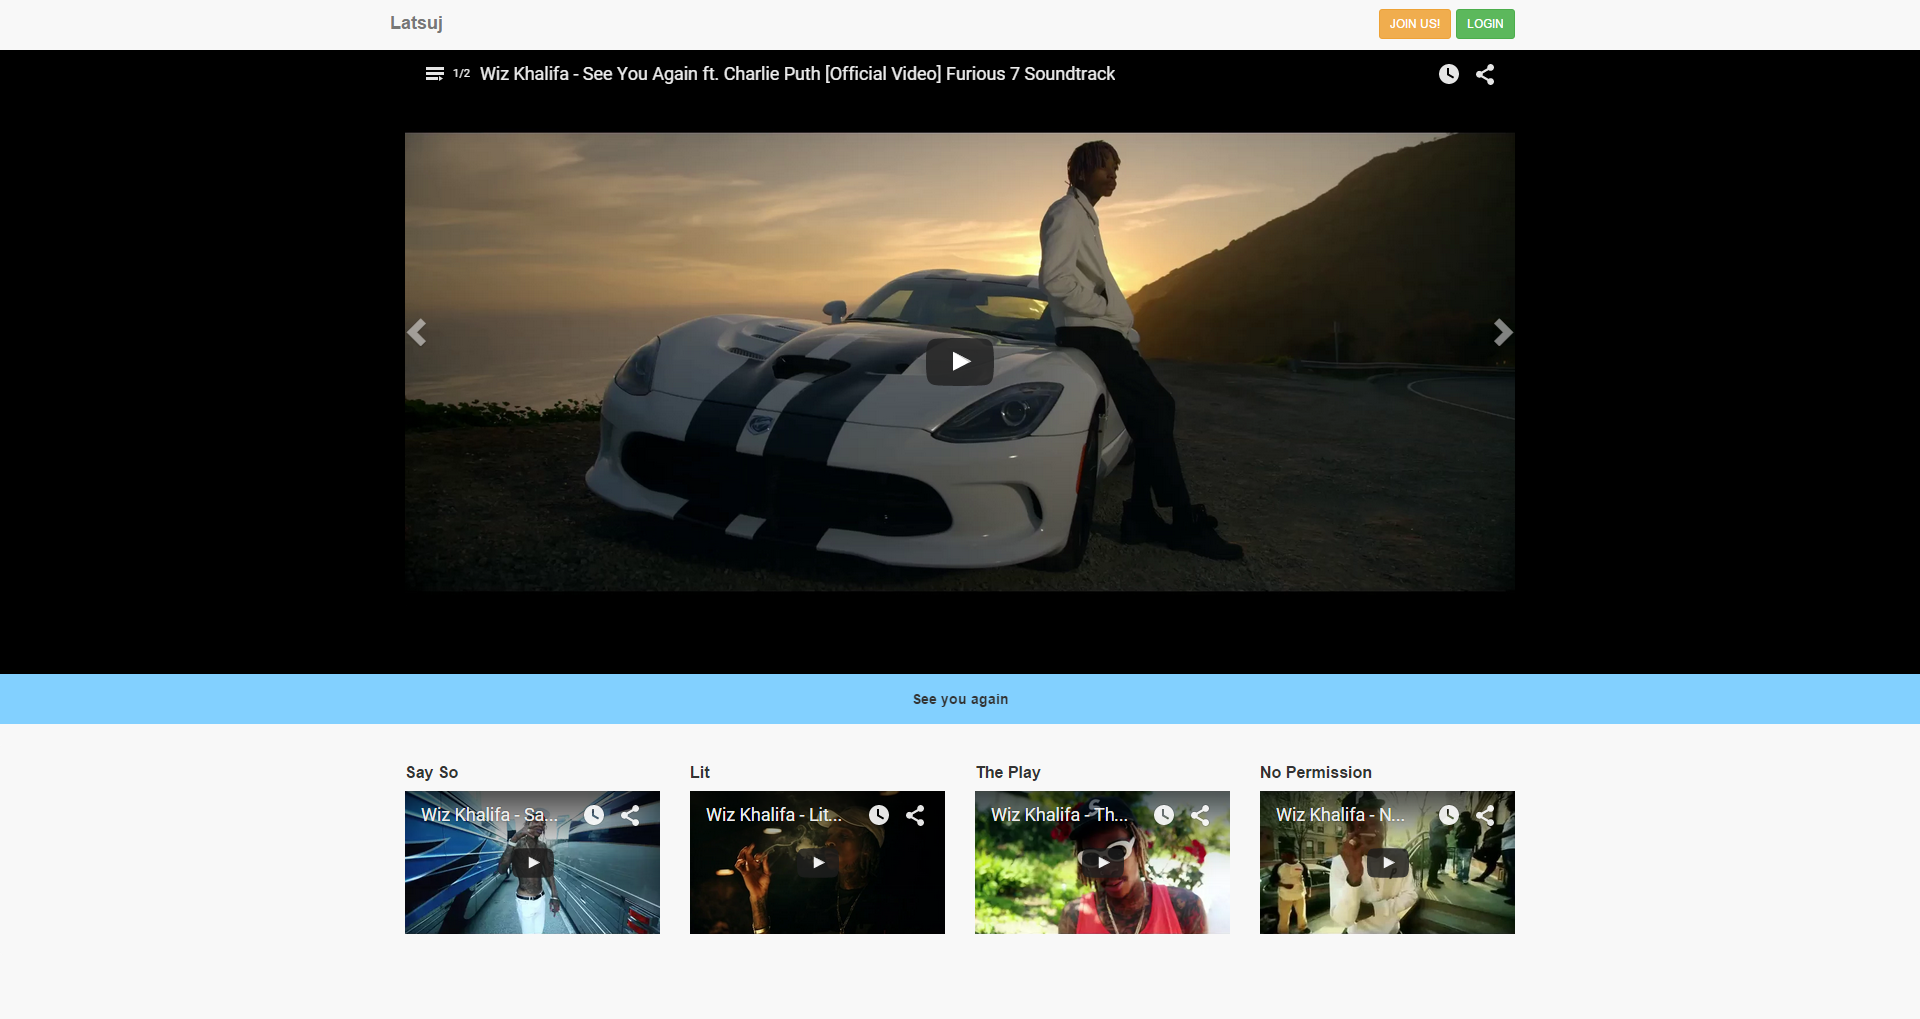
\includegraphics[width=1.0\textwidth]{pc}\\
\vspace{3cm}
\textbf{\Large{JUSTAL KEVIN}}\\
2015\\
\vspace{2cm}
\textbf{Justal Kevin - \color{blue}{\underline{justal@polytech.unice.fr}} \color{black}{- SI5 - IHM}}\\
\vspace{4cm}
\textbf{Enseignant :}\\
\textbf{Anne Marie Dery - \color{blue}{\underline{dery@polytech.unice.fr}}}
\end{center}

\newpage
\newpage
\tableofcontents

\newpage

\section{Comment avez vous r\'ealis\'e l'exemple ?}

\begin{wrapfigure}{r}{0.5\textwidth}
  \vspace{-20pt}
  \begin{center}
    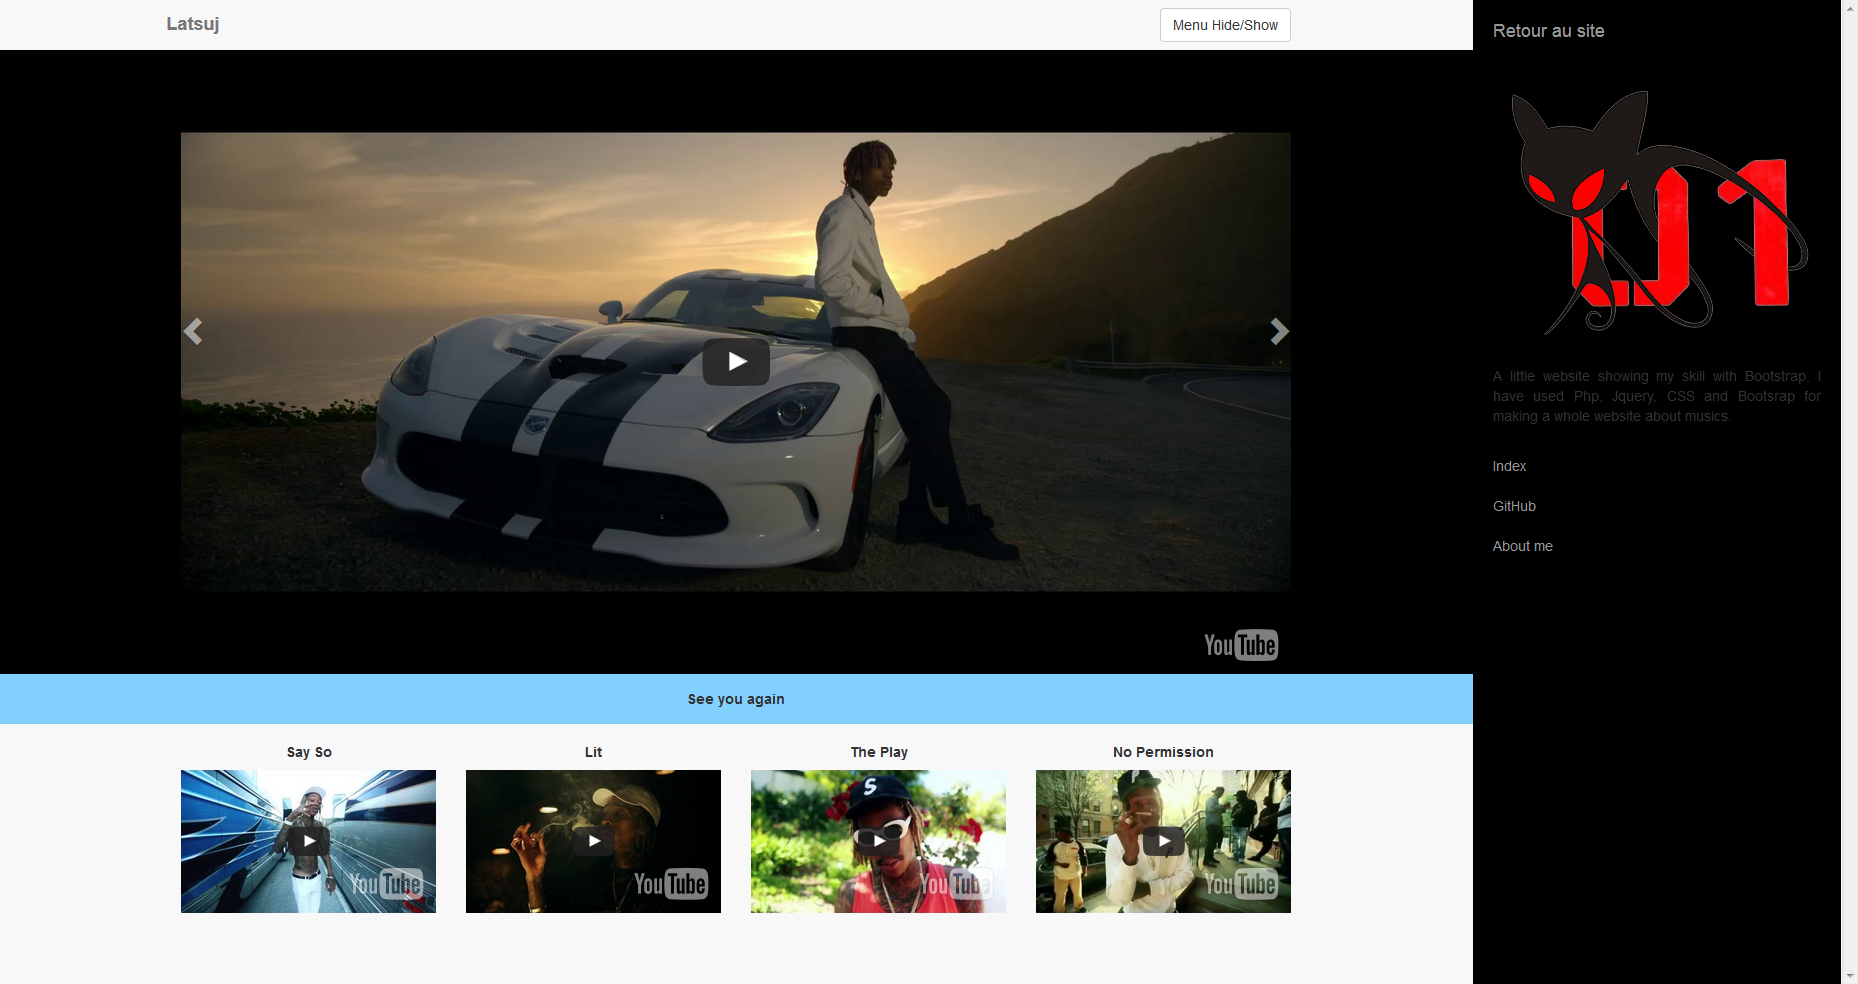
\includegraphics[width=0.48\textwidth]{p2}
  \end{center}
  \vspace{-20pt}
  \caption{Le site pour PC}
  \vspace{-10pt}
\end{wrapfigure}

Pour r\'ealiser mon exemple, je me suis dans un premier temps int\'eress\'e \`a la d\'efinition m\^eme d'un site web adaptatif. Le principe du RWD (\textit{responsive web design}) ou site web adaptatif dans la langue de moli\'ere consiste \`a s'appuyer sur l'usage des \textit{Media queries} que l'on peux aussi appeler \og points de rupture \fg , de grilles de positionnement et d'images flexibles pour rendre un site adaptable \`a son support.\\
Pour d\'evelopper, je suis parti de la version ordinateur \`a une taille relativement imposante, puis j'ai remis en forme les \'el\'ements \`a mesure que la largeur de l'\'ecran diminuait voire je les supprimais totalement. J'ai essay\'e autant que faire se peut d'ajouter un maximum d'\'el\'ements diff\'erents. On retrouve ainsi des vid\'eos, un menu, des tableaux, des images, du texte, des \'el\'ements interactifs comme des boutons... Il y a donc l'ensemble des \'el\'ements que l'on peux retrouver sur n'importe quels sites lambda. \\

\subsection{Structure du site}

\begin{wrapfigure}{l}{0.5\textwidth}
  \vspace{-20pt}
  \begin{center}
    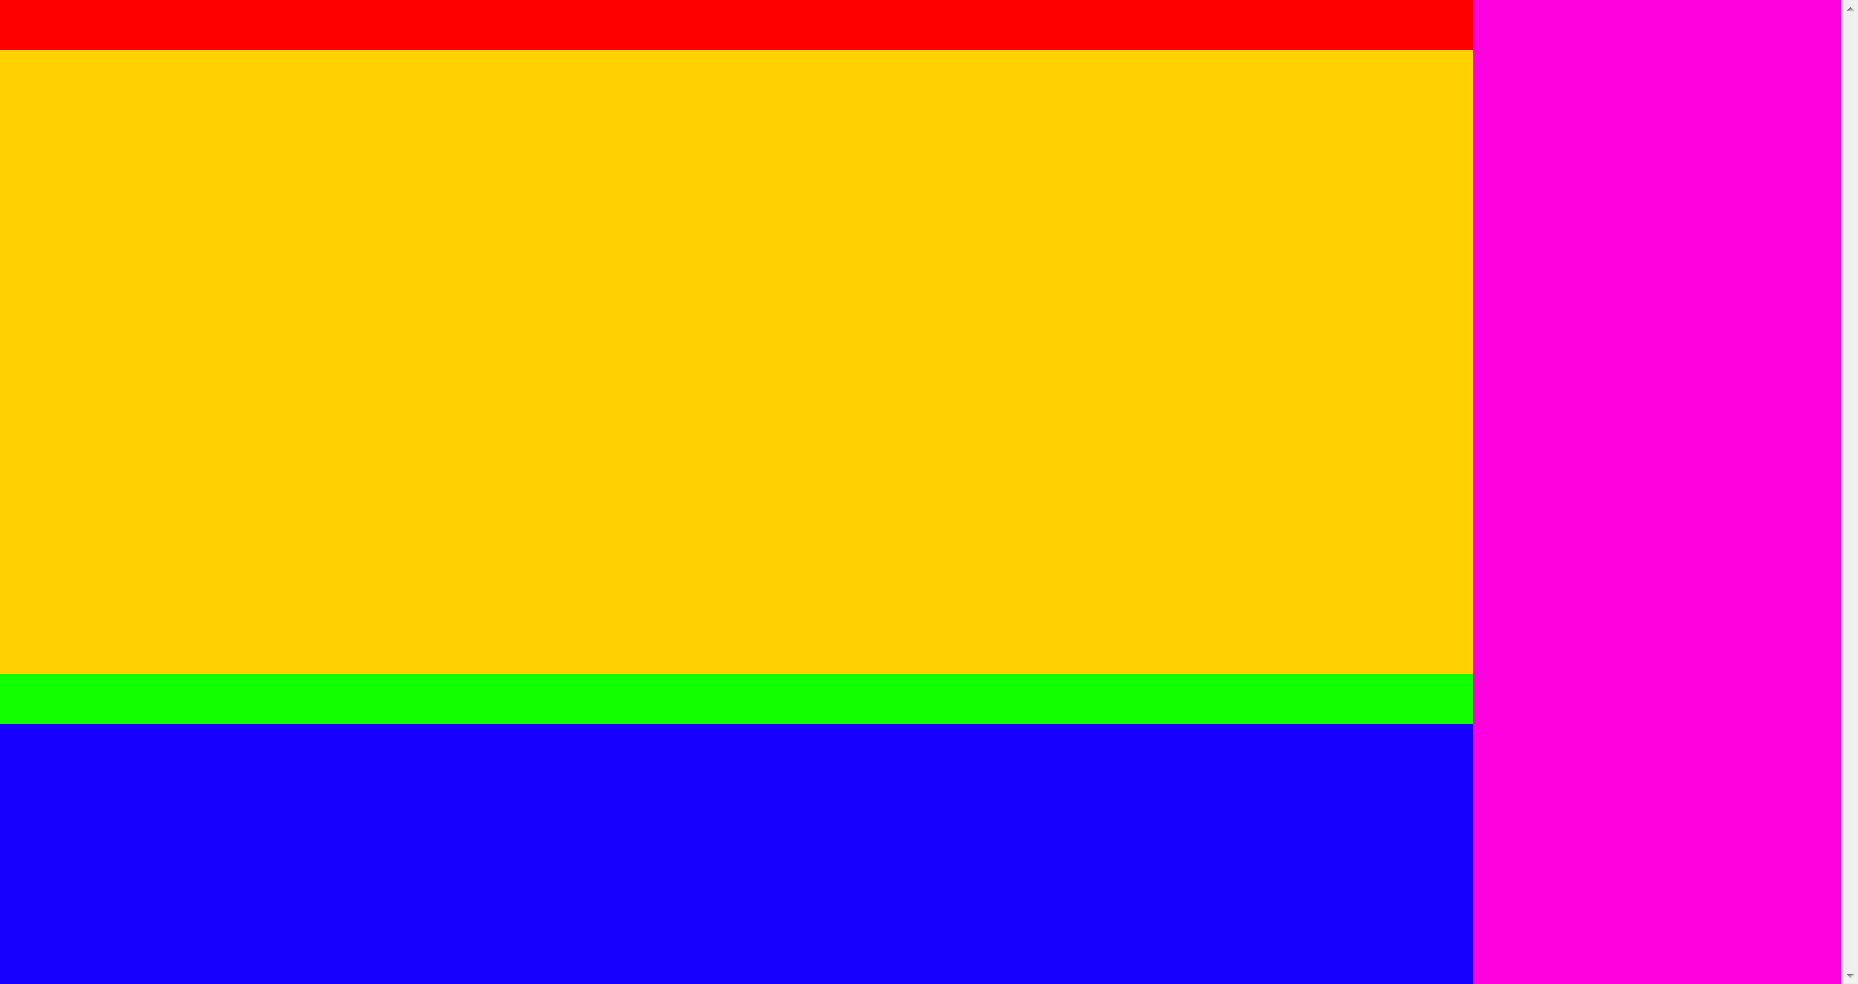
\includegraphics[width=0.48\textwidth]{p3}
  \end{center}
  \vspace{-20pt}
  \caption{Structure du site}
  \vspace{-10pt}
\end{wrapfigure}

Les deux technologies que j'ai choisie partage la m\^eme structure de base. C'est \`a dire un d\'ecoupage en cinq grands blocs. Sur la figure 2, le bloc en rouge repr\'esente la barre principale. En jaune, on retrouve la zone de lecture principale des clips musicaux. En vert, il s'agit d'un bouton permettant d'ouvrir un bloc d'information concernant le clip de la zone jaune. En bleu, il s'agit simplement d'autres clips musicaux en rapport avec le chanteur chantant dans le clip de la zone jaune. En rose, on retrouve un menu que l'on peux ou non affich\'e gr\^ace \`a un bouton se trouvant dans la zone rouge. Si le menu est rentr\'e, la zone violet n'existe plus et on se retrouve avec seulement quatres blocs qui prendront la totalit\'e de la fen\^etre comme on peux l'observ\'e sur l'image suivante :\\

\begin{center}
  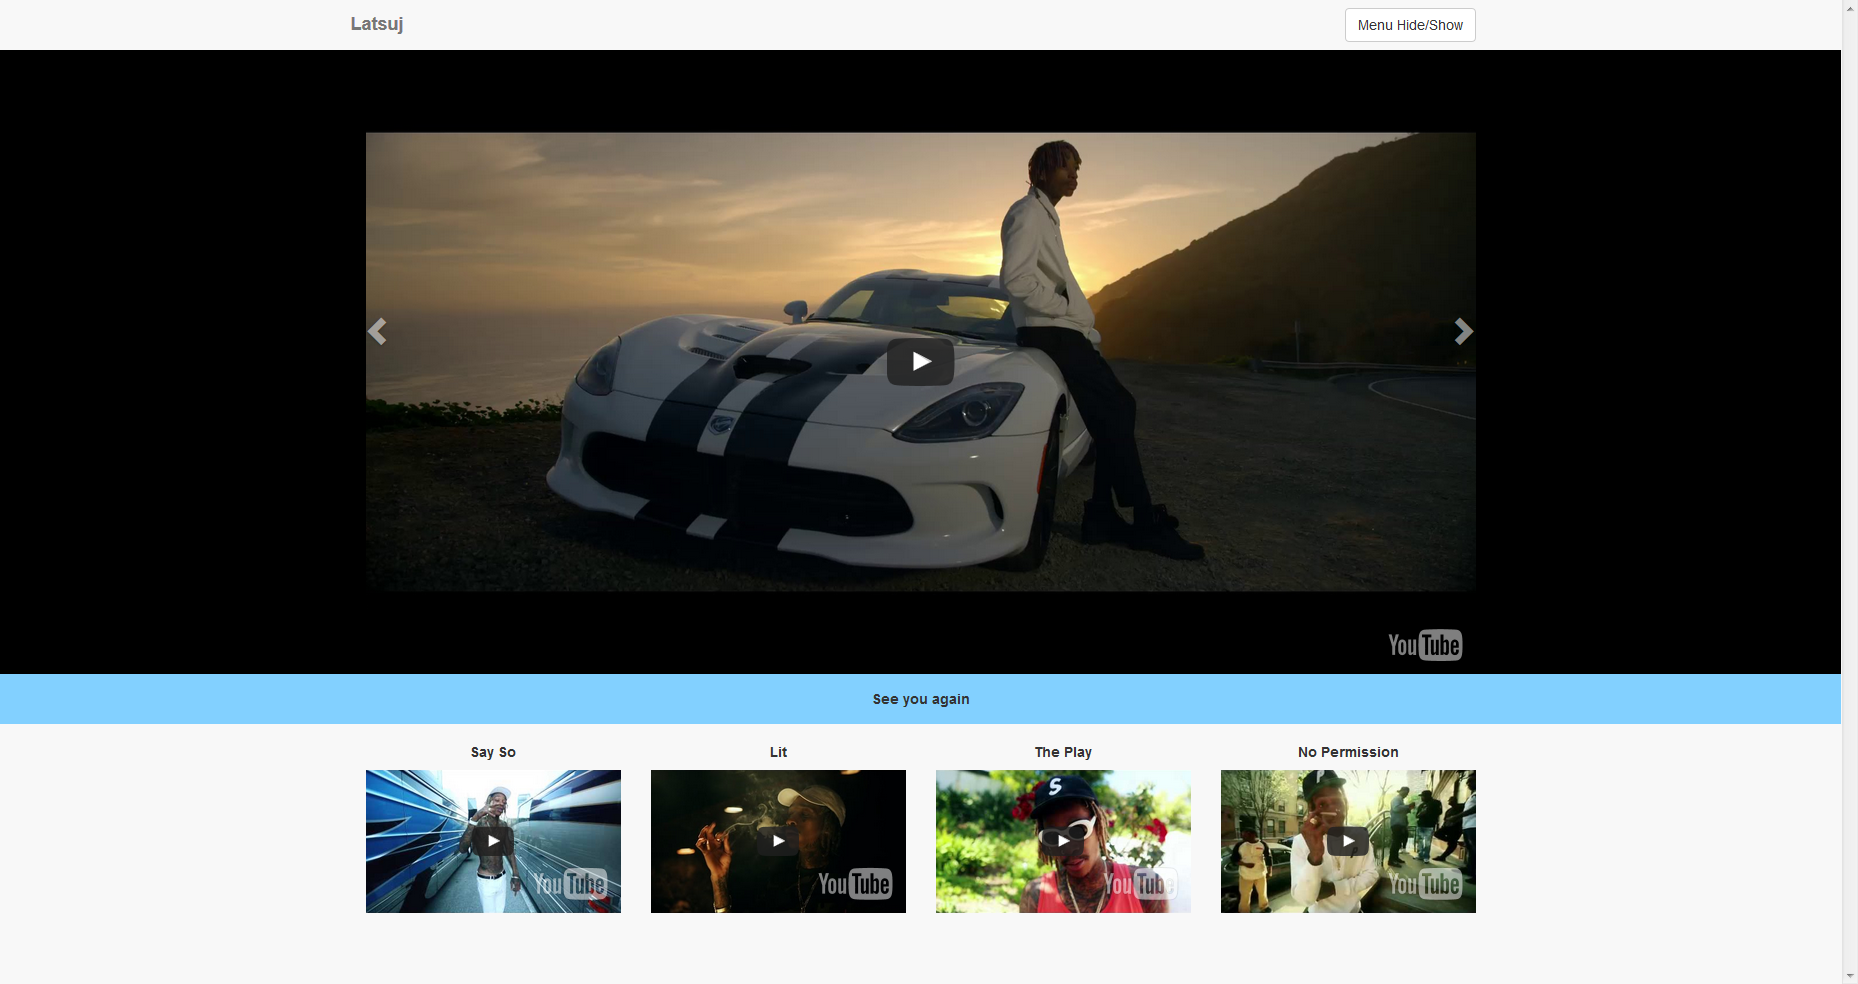
\includegraphics[width=0.8\textwidth]{p1}
\end{center}

\subsection{Images flexibles}

Pour observer pr\'ecis\'ement les diff\'erents principes de RWD sur notre site, nous allons nous int\'erresser \`a certaines zones du site. Pour commencer, nous allons d'abord nous int\'eress\'e au menu (zone violet). Cette derni\'ere illustre \`a la perfection le principe d'image flexible que l'on attend d'un site adaptatif. Qu'est ce qu'une image flexible ? Il s'agit d'une image qui se redimensionnera en fonction de la taille de la fen\^etre. Pour r\'ealiser cela, il faut simplement donner \`a une image quelques attributs CSS. Il faut lui sp\'ecifi\'e de prendre toute la longueur disponible dans le bloc o\`u elle se trouve et de prendre une hauteur automatiquement en fonction de son rapport. En CSS, cela se traduit par : \textit{\og width:100\%;height:auto; \fg{} }. Avec Polymer, j'ai cr\'e\'e un object image qui ajoutait automatiquement des images responsives. Sous Bootstrap, c'est on ne peux plus simple, une classe existe nomm\'e \textit{\og img-responsive \fg} et il suffit de la rajouter sur une balise IMG. Cela permet d'obtenir le r\'esultat suivant lorsque l'on r\'eduit la taille de la fen\^etre :\\

\begin{center}
  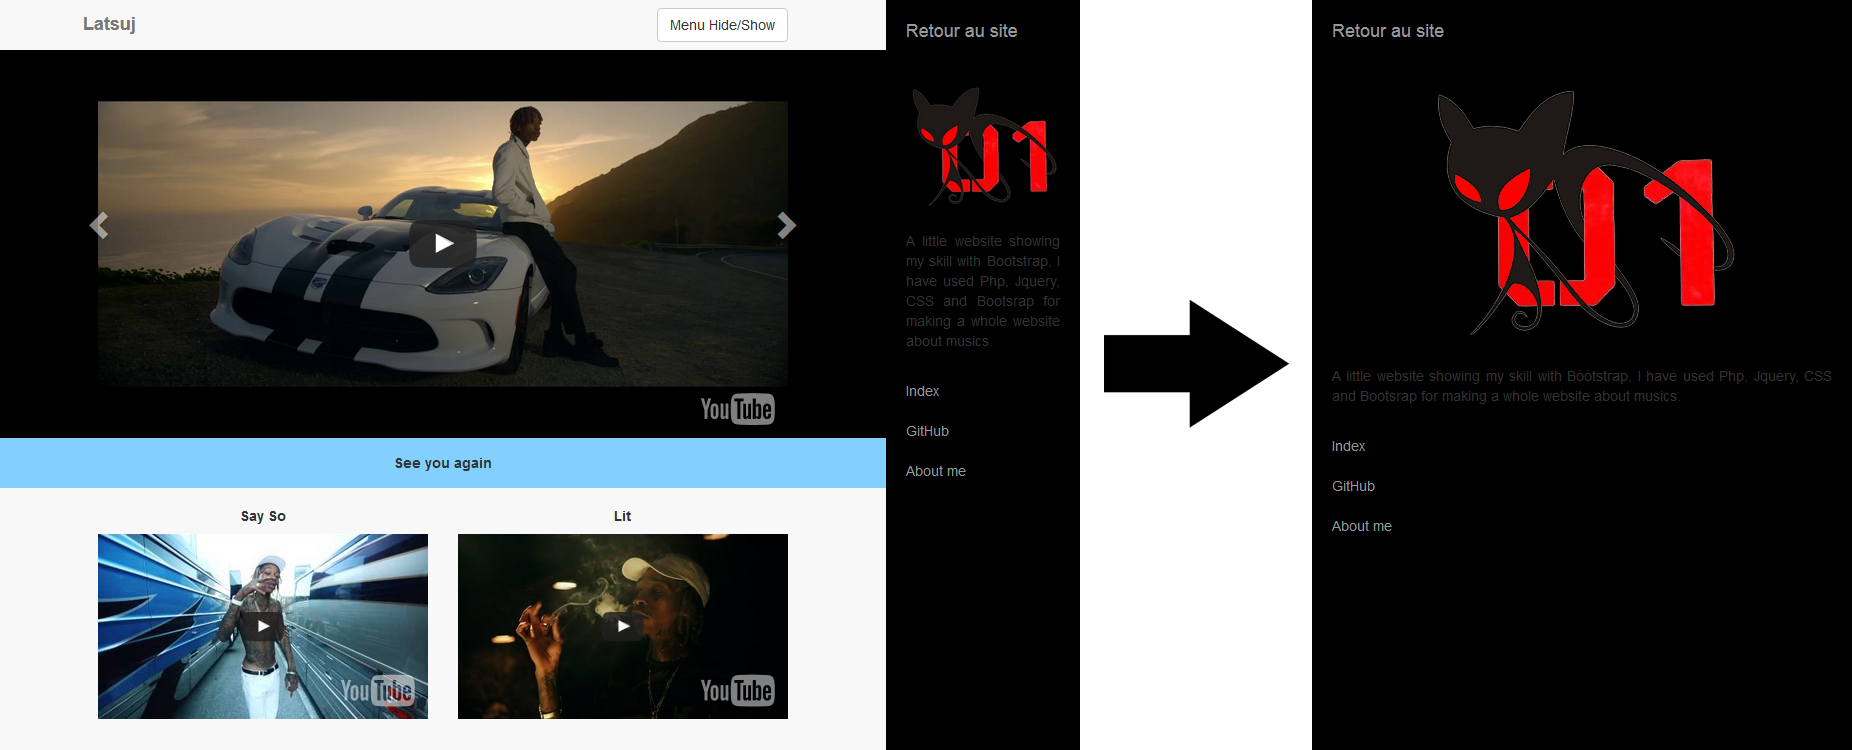
\includegraphics[width=0.8\textwidth]{p4}
\end{center}

Dans mon exemple ci-dessus, on remarque bien que l'image s'adapte \`a la taille de la fen\^etre. On remarque de plus que le site est totalement diff\'erent, il s'agit l\`a de l'application des points de rupture ou Media queries dont je parlais pr\'ec\'edemment et que nous allons voir au prochain point.

\subsection{Media queries ou Points de rupture}

Les \textbf{media queries} ou points de rupture sont des r\`egles CSS appliqu\'ees en fonction de la largeur de l'\'ecran. Ce sont ces diff\'erentes largeurs qui sont appel\'ees \og points de rupture \fg{}, elles correpondent \`a un besoin de modifier la page \`a partir d'un seuil critique pour la facilitation de la navigation et de la lecture du contenu. Pour que cette d\'efinition soit clair, nous allons montrer leur application sur le site. \\

\begin{wrapfigure}{l}{0.5\textwidth}
  \vspace{-20pt}
  \begin{center}
    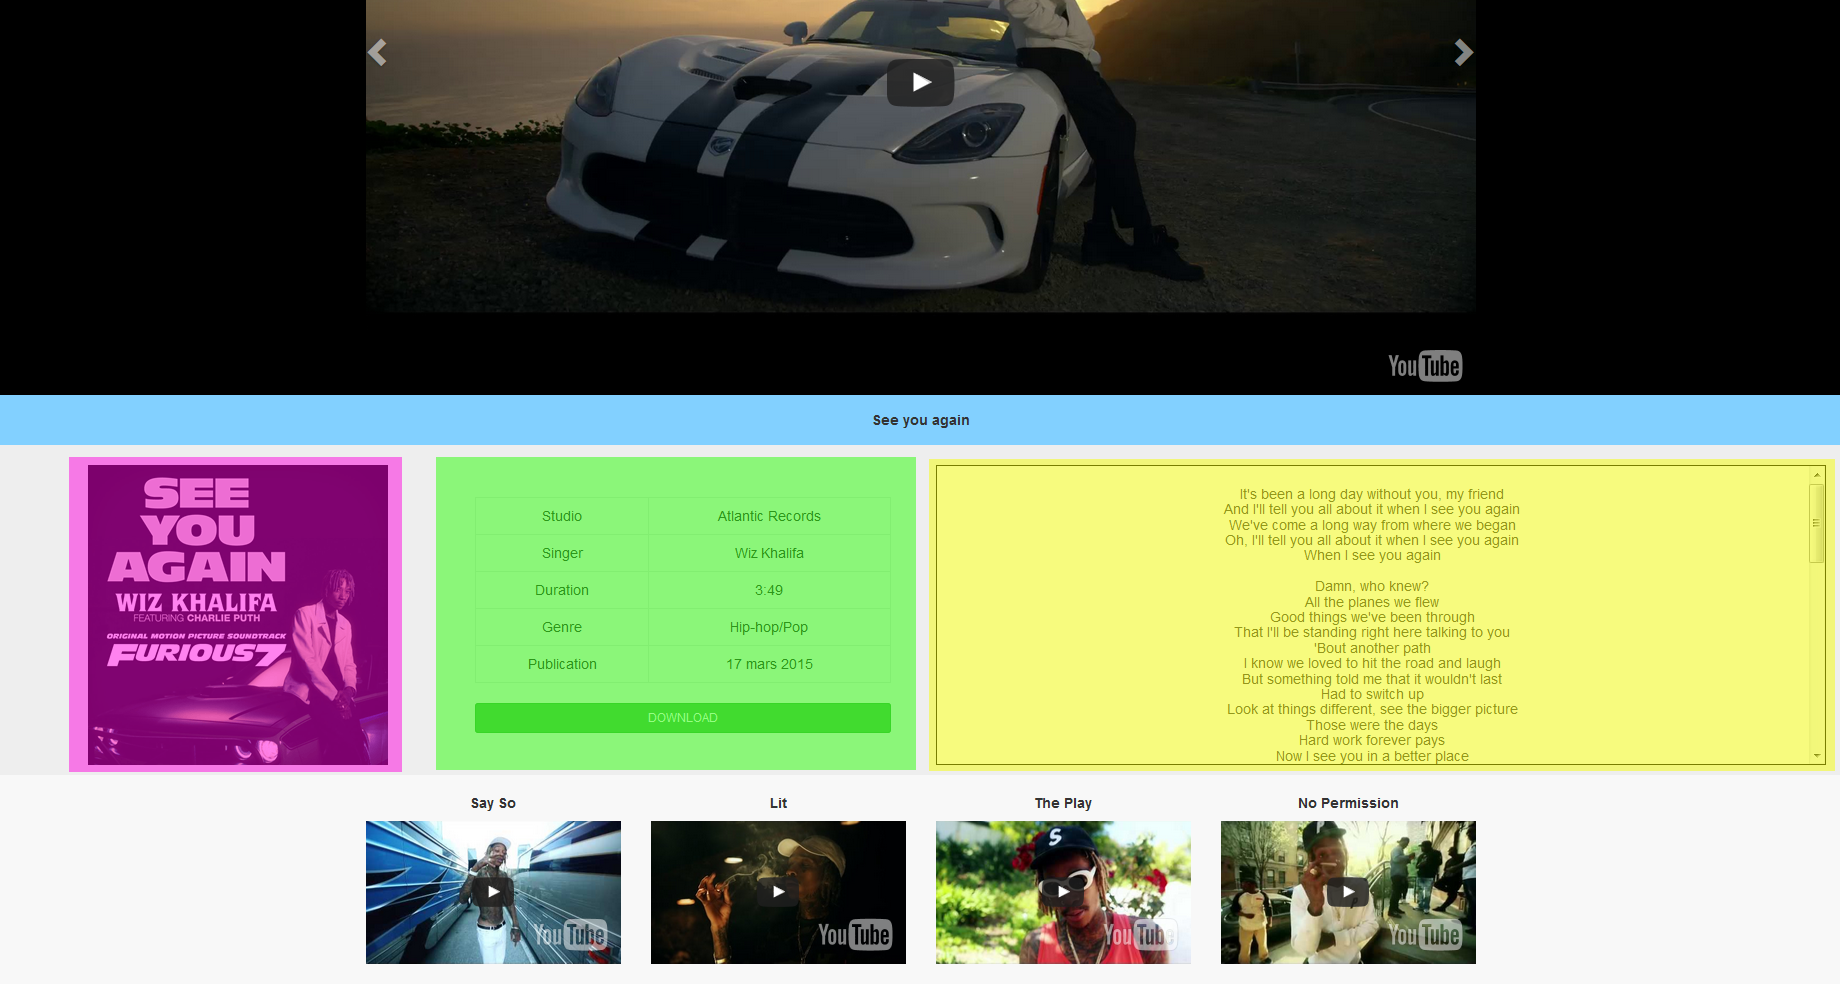
\includegraphics[width=0.48\textwidth]{p5}
  \end{center}
  \vspace{-20pt}
  \caption{Les blocs}
  \vspace{-10pt}
\end{wrapfigure} 

Sur la figure 3, j'ai colori\'e les diff\'erents blocs chacun d'une couleur diff\'erente. Ces blocs sont simplements repr\'esent\'es par des balises DIV avec des r\`egles CSS fonction de la taille de l'\'ecran. Prenons l'exemple du bloc violet, ce bloc fait exactement 25\% du conteneur qui lui prend 100\% de la longueur de l'\'ecran. Lorsque l'on r\'eduit la fen\^etre jusqu'\`a un certain point, ce bloc prendra alors 50\% sur ces 100\%. Puis si l'on continue \`a r\'eduire la fen\^etre, ce bloc disparait.\\  

\begin{center}
  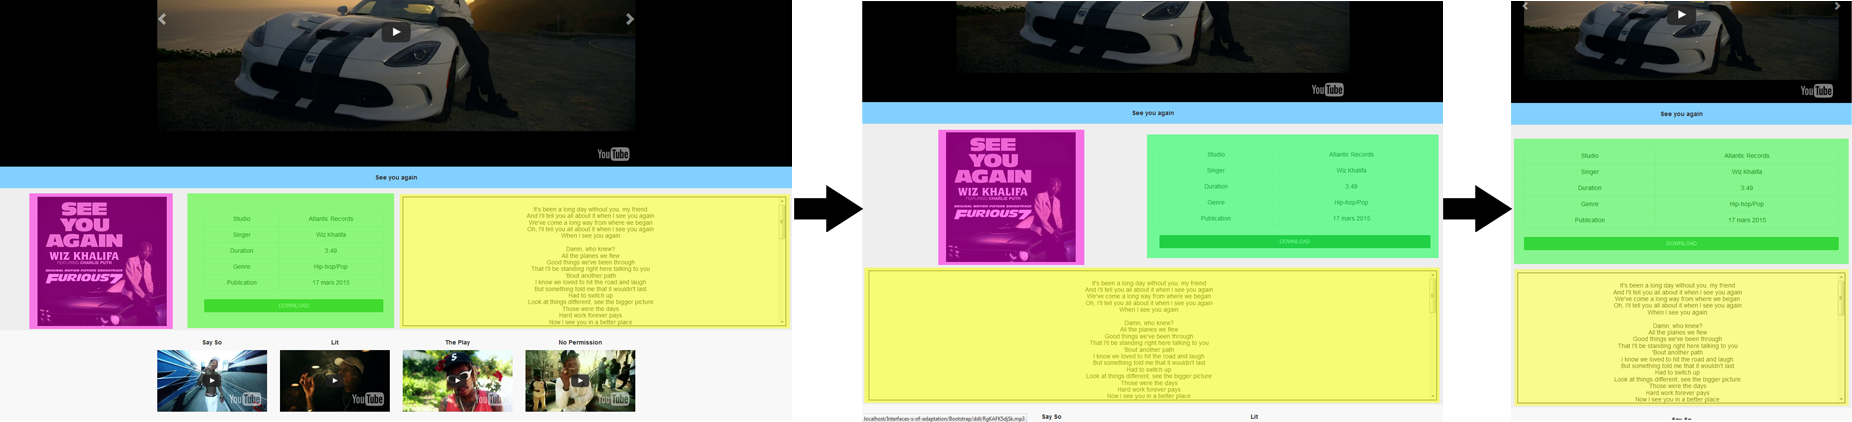
\includegraphics[width=0.8\textwidth]{p8}
\end{center}

Sur Bootstrap, il est assez simple de r\'ealiser ceci. Cet technologie inclue un syst\`eme de grille relativement bien ficell\'e. Il faut dans un premier temps, d\'efinir notre zone o\`u on souhaite r\'ealiser le d\'ecoupage en utilisant la classe \og container \fg{} dans une balise DIV :
\vspace{0.5cm}\\
\fbox{\parbox{\textwidth}{<div class="container">\\
</div>}}
\vspace{0.5cm}
\begin{wrapfigure}{r}{0.5\textwidth}
  \vspace{-20pt}
  \begin{center}
    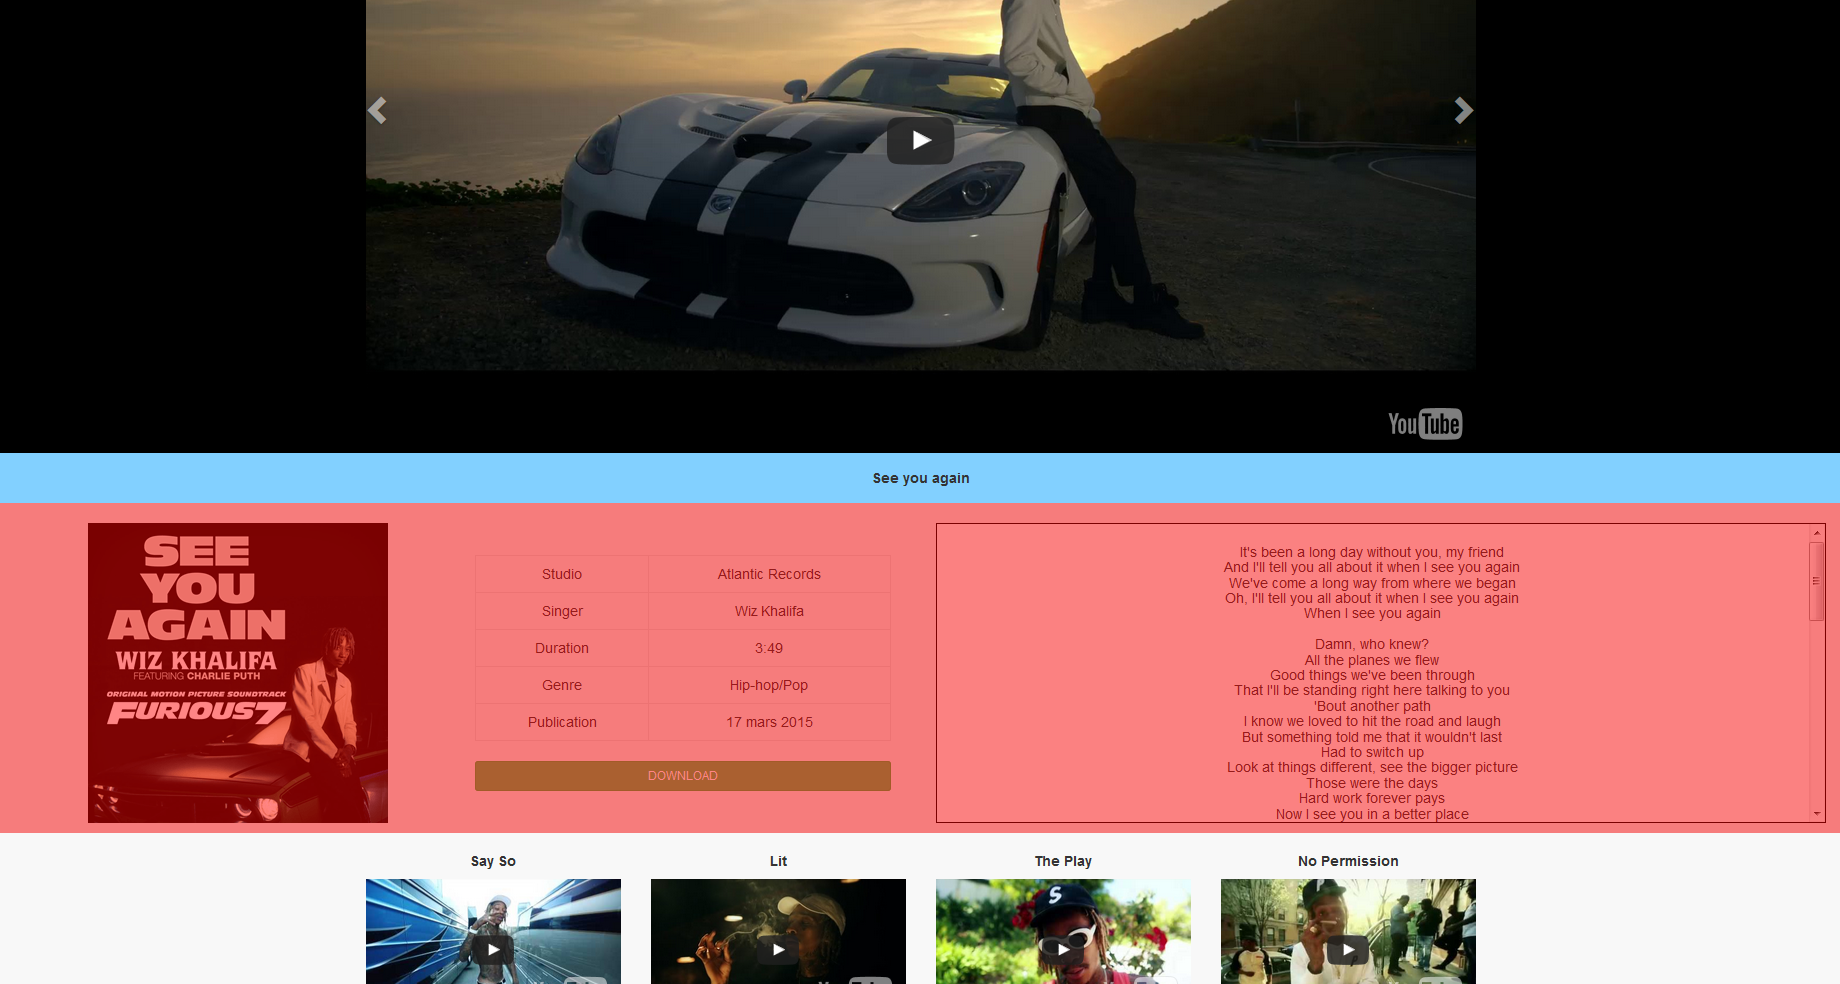
\includegraphics[width=0.48\textwidth]{p9}
  \end{center}
  \vspace{-20pt}
  \caption{Zone du container}
  \vspace{-10pt}
\end{wrapfigure} 
\hspace*{0.6cm}On a ainsi sp\'ecifi\'e o\`u se trouvait notre zone par dessus laquelle nous allons poser une grille. J'entrerais dans les d\'etails au chapitre suivant, pour l'instant il faut voir cela comme une subdivision en 12 partie de la partie rouge sur la figure 4. Comme je l'ai d\'ej\`a sp\'ecifi\'e pr\'ec\'edement, l'image dans la partie rouge ne repr\'esente que 25\% de cette zone lorsque l'\'ecran est sup\'erieur \`a 1500px (valeur choisie par mes soins). Pour ensuite, sp\'ecifi\'e \`a Bootstrap que nous allons couper notre container en plusieurs parties, il faut utiliser la classe \og row \fg{} : 
\vspace{0.5cm}\\
\fbox{\parbox{\textwidth}{<div class="container">\\
\hspace*{0.6cm}<div class="row">\\
\hspace*{0.6cm}</div>\\
</div>}}
\vspace{0.5cm}\\
Nous allons maintenant entrer dans le vif du sujet, comme dit plus haut, le container est divis\'e en 12 parties que j'appellerais dans la suite colonne. On peux fixer le nombre de colonne que peux prendre un \'el\'ement. Reprenons et analysons pr\'ecisement la figure 3. Sur cette derni\`ere, la zone jaune prend 6 colonnes et les 6 colonnes restantes sont r\'eparties \'equitablement entre la zone violette et verte. Niveau code, on sp\'ecifie cela en utilisant les classes \og col-xs-X \fg,\og col-sm-X \fg,\og col-md-X \fg ou \og col-lg-X \fg. Xs, sm, md et lg repr\'esentent la taille minimum de l'\'ecran pour que les r\`egles que ces classes contiennent prennent effets. Tandis que le X dans ces classes repr\'esente tout simplement le nombre de colonnes que prendra l'\'el\'ement utilisant ces classes. Je reviendrais un peu plus loin sur ce point, pour l'instant, il est plus important de comprendre la diff\'erence entre les classes xs, sm, md et lg :
\vspace{0.5cm}\\
\fbox{\parbox{\textwidth}{<div class="container">\\
\hspace*{0.6cm}<div class="row">\\
\textbf{\hspace*{1.2cm}\color{red}{<div class="col-md-12 col-lg-6">}}\\
\hspace*{1.8cm}<div class="row">\\
\textbf{\hspace*{2.4cm}\color{blue}{<div class="hidden-xs hidden-sm col-md-6 col-lg-6>}}\\
\hspace*{3.0cm}...\\
\hspace*{2.4cm}</div>\\
\hspace*{2.4cm}...\\
\hspace*{1.8cm}</div>\\
\hspace*{1.2cm}</div>\\
\hspace*{1.2cm}...\\
\hspace*{0.6cm}</div>\\
</div>}}
\vspace{0.5cm}\\
Ce bout de code est suffisant pour comprendre et expliqu\'e clairement les mouvements de l'image violette dans la figure 3. Le texte en rouge pr\'ecise qu'\`a grande taille lg (sup\'erieur \`a 1500px), la zone violette et verte ont 50\% du container, soit 6 colonnes : \og col-lg-6 \fg{} . Le texte en bleu est la balise DIV directe qui contient l'image violette. Ces classes sp\'ecifies qu'\`a grande taille, ce bloc ne peux exc\'eder 6 colonnes, soit 50\%. Or, 50\% de 50\% fait bien 25\% comme je l'avais dit plus haut. Cependant cela n'est valide que lorsque la fen\^etre est sup\'erieur \`a 1500px. En dessous, les autres classes prennent le relais.\\ 

\begin{wrapfigure}{r}{0.5\textwidth}
  \vspace{-20pt}
  \begin{center}
    \begin{tabular*}{0.48\textwidth}{@{\extracolsep{\fill}} | c | l | }
  \hline
  xs & 600px\\
  \hline
  sm & 900px\\
  \hline
  md & 1200px\\
  \hline
  lg & 1500px\\
  \hline
\end{tabular*}
  \end{center}
  \vspace{-20pt}
  \caption{Points de rupture}
  \vspace{-10pt}
\end{wrapfigure} 

Pour comprendre pr\'ecisement quelles sont les classes qui sont actives \`a une grandeur de fen\^etre donn\'e, il faut simplement retenir les dimensions que repr\'esentent les sigles xs, sm, md, lg. Les dimensions qui sont affich\'ees ne sont pas celles par d\'efauts de BootStrap mais celles que j'ai utilis\'e pour mon site. J'ai chang\'e les points de rupture pour que mon menu puisse s'ins\'errer joliment sur mon site. Sans cela, il se pouvait que le bouton de la barre de menu chevauche le menu, ce qui donnait un r\'esultat pl\^utot moche. La seule mani\`ere de r\'egler le probl\`eme a \'et\'e de construire une version personnalis\'e de Boostrap. Il est possible d'\'effectuer cette op\'eration sur le site officiel de Bootstrap.\\

\begin{wrapfigure}{l}{0.5\textwidth}
  \vspace{-20pt}
  \begin{center}
    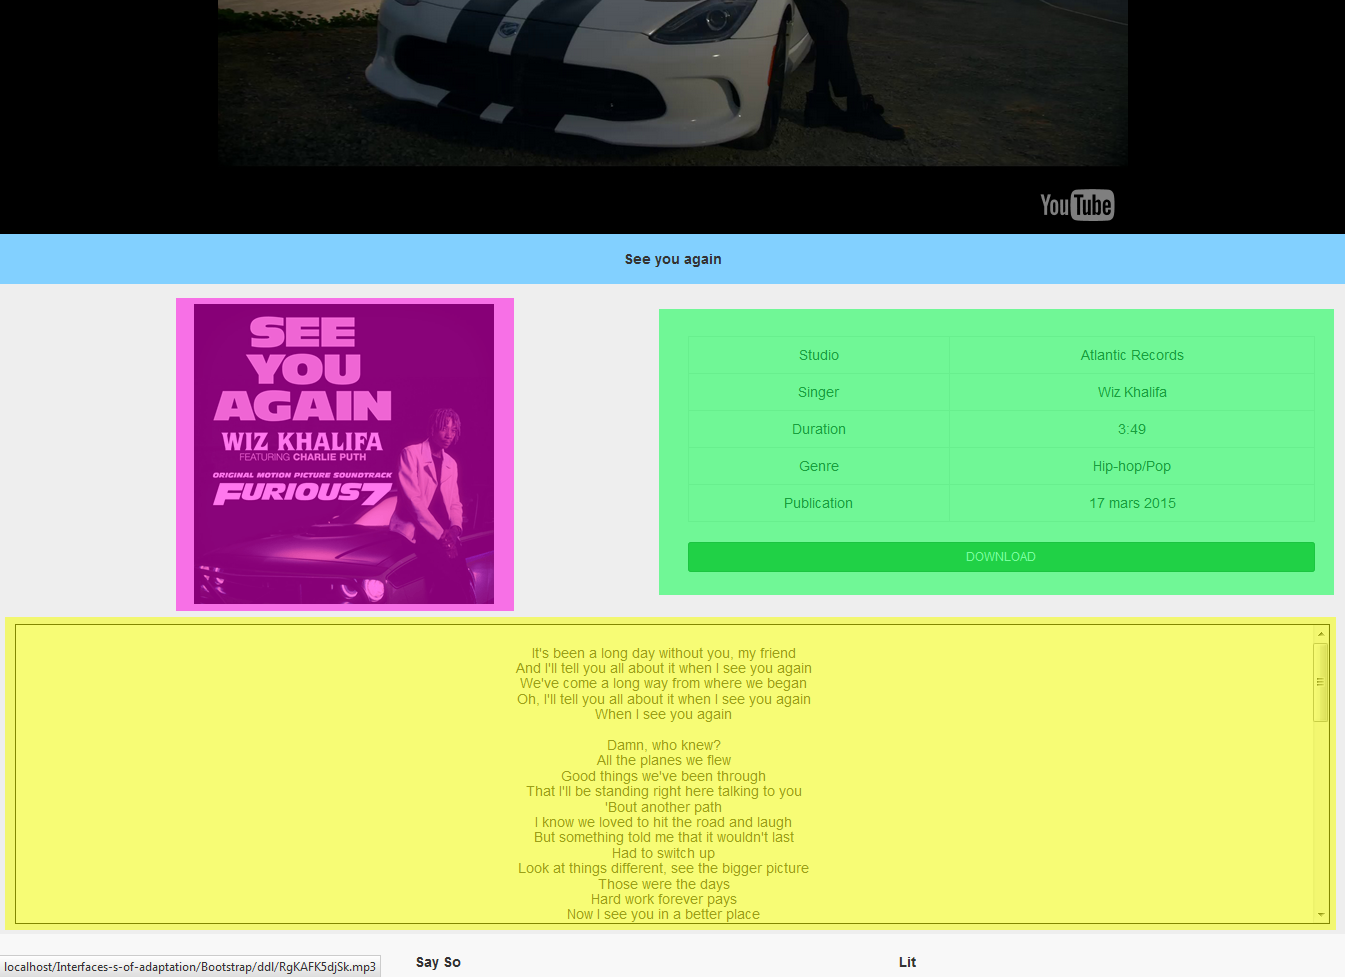
\includegraphics[width=0.48\textwidth]{p6}
  \end{center}
  \vspace{-20pt}
  \caption{50\% de la fen\^etre}
  \vspace{-10pt}
\end{wrapfigure} 

Dans notre cas, si la fen\^etre est inf\'erieur \`a 1500px alors les classes lg ne sont plus utilis\'e. Prenons une fen\^etre de 1300px, si l'on regarde le tableau de la figure 5, on remarque que pour toutes les dimensions situ\'es entre 1200 px et 1500 px md est la classe qui est actif. On reprend notre bout de code pr\'ec\'edent et on remarque que le texte en rouge mentionne \og col-md-12 \fg{}. Cela signifie que cette div qui repr\'esente la zone violette et verte de la figure 3 prendra 100\% du container. On regarde notre texte en bleu et on lit \og col-md-6 \fg{}. L'image violette prendra donc 50\% de 100\%, elle prendra donc la moiti\'e de la longueur de la fen\^etre.\\

\begin{wrapfigure}{l}{0.5\textwidth}
  \vspace{-20pt}
  \begin{center}
    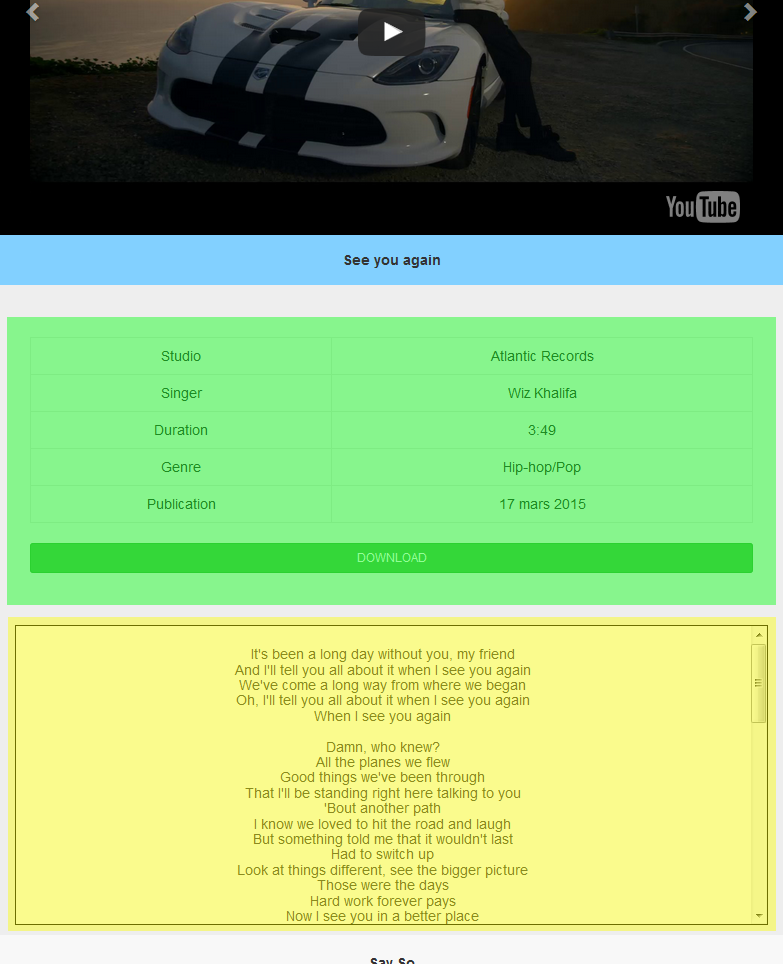
\includegraphics[width=0.48\textwidth]{p7}
  \end{center}
  \vspace{-20pt}
  \caption{L'image a disparu}
  \vspace{-10pt}
\end{wrapfigure} 

Maintenant, si nous continuons de r\'eduire la fen\^etre et atteignons une taille inf\'erieur \`a 1200px, nous arrivons dans les classes sm. Si on regarde le texte en bleu dans le bout de code pr\'ec\'edent, on voit qu'il est \'ecrit \og hidden-sm \fg{}. Cette classe signifie que le nombre de colonne prise par cet \'el\'ement sera r\'eduit \`a z\'ero. Cela se traduit par une disparition compl\`ete de l'\'el\'ement comme on peux le voir sur la figure 7. Notons au passage que je n'ai pas pr\'ecis\'e dans le texte en rouge le nombre de colonne pour les dimensions sm et xs. Je n'ai pas eu \`a le faire car Bootstrap utilise les r\`egle CSS pour r\'ealiser ces modifications. Plus pr\'ecisement, Bootstrap utilise l'h\'eritage et le cascading de CSS pour pouvoir r\'e\'ecrire des r\`egles sur des r\`egles. Si on ne d\'efini pas de xs, alors les r\`egles CSS seront celles de sm. Si elles aussi ne sont pas d\'efinis, alors ce seront celles de md qui seront prise en compte...Cela ne constitue pas une faute mais j'aurais pu omettre le \og col-md-6 \fg{} dans mon texte bleu et cela donnerais toujours le m\^eme r\'esultat.\\

Nous avons vu comment mettre cela en place sur Bootstrap, on peux \'evidemment faire la m\^eme chose avec Polymer. Le r\'esultat obtenue est le m\^eme mais la mani\`ere d'y arriver est diff\'erente. Cependant, notons que cela est totalement contraire \`a l'id\'ee de Polymer. J'ai discut\'e de cela avec Monsieur Bidelman lui-m\^eme qui est un des fondateurs de Polymer et qui travaille actuellement chez Google. Le but est de cr\'eer des \'el\'ements r\'eutilisables. Or \`a partir du moment o\`u l'on utilise des m\'edias queries, l'\'el\'ement devient ancr\'e au site qui les utilisent. Prenons l'exemple pr\'ec\'edent, pour que l'image disparaisse \`a un certain point de rupture, j'ai cr\'e\'e un \'el\'ement qui change son attribut \og display \fg{} lorsque l'on atteint ce fameux point.
\vspace{0.5cm}\\
\fbox{\parbox{\textwidth}{
<dom-module id="my-col-hidden-900">\\
\hspace*{0.6cm}<template>\\
\hspace*{1.2cm}<style>\\				
\hspace*{1.8cm}\color{blue}{@media (max-width:900px) \{\\
\hspace*{2.4cm}:host \{\\
\hspace*{3.0cm}display: none;\\
\hspace*{2.4cm}\}\\
\hspace*{1.8cm}\}\\
\hspace*{1.2cm}}\color{black}{</style>\\
\hspace*{1.2cm}<content></content>\\
\hspace*{0.6cm}</template>\\
\hspace*{0.6cm}<script>\\
\hspace*{1.2cm}Polymer({\\
\hspace*{1.8cm}is: "my-col-hidden-900"\\
\hspace*{1.2cm}});\\
\hspace*{0.6cm}</script>\\
</dom-module>}}}
\vspace{0.5cm}\\
On a donc cr\'e\'e une nouvelle node HTML nomm\'e my-col-hidden-900. Le code en bleu est la partie la plus importante. Elle sp\'ecifie que le code se situant entre les balises \og my-col-hidden-900 \fg{} aura l'attribut \og display:none \fg{} si la taille de la fen\^etre est inf\'erieur \`a 900px. Autrement dit, tous le contenue \`a l'int\'erieur ne sera pas affich\'e.\\
Dans le m\^eme style, j'ai cr\'e\'e un \'el\'ement du DOM dont la longueur s'adapte en fonction la largeur de la fen\^etre. La longueur ainsi que le position naturel des balises DIV avec l'attribut \og float:left \fg{} permet de r\'ealiser un semblant de grille sous Polymer :
\vspace{0.5cm}\\
\fbox{\parbox{\textwidth}{
<dom-module id="my-col-25-100">\\
\hspace*{0.6cm}<template>\\
\hspace*{1.2cm}<style>\\
\hspace*{1.8cm}\color{blue}{:host \{	\\	
\hspace*{2.4cm}position: relative;\\
\hspace*{2.4cm}min-height: 1px;\\
\hspace*{2.4cm}padding-left: 15px;\\
\hspace*{2.4cm}padding-right: 15px;\\
\hspace*{2.4cm}float:left;\\
\hspace*{2.4cm}width:25\%;\\
\hspace*{2.4cm}box-sizing: border-box;\\
\hspace*{1.8cm}\} }\\
\hspace*{1.8cm}\color{red}{@media (max-width:1500px) \{\\
\hspace*{2.4cm}:host \{\\
\hspace*{3.0cm}width:50\%;\\
\hspace*{2.4cm}\}\\
\hspace*{1.8cm}\}}	\\	
}}\\
\fbox{\parbox{\textwidth}{
\hspace*{1.8cm}\color{green}{@media (max-width:900px) \{\\
\hspace*{2.4cm}:host \{\\
\hspace*{3.0cm}width:100\%;\\
\hspace*{2.4cm}\}\\
\hspace*{1.8cm}\}}		\\
\hspace*{1.8cm}\color{black}{</style>\\
\hspace*{1.8cm}<content></content>\\
\hspace*{0.6cm}</template>\\
\hspace*{0.6cm}<script>\\
\hspace*{1.2cm}Polymer(\{\\
\hspace*{1.8cm}is: "my-col-25-100"\\
\hspace*{1.2cm}\});\\
\hspace*{0.6cm}</script> \\ 
</dom-module>}}}
\vspace{0.5cm}\\

\begin{wrapfigure}{r}{0.5\textwidth}
  \vspace{-20pt}
  \begin{center}
    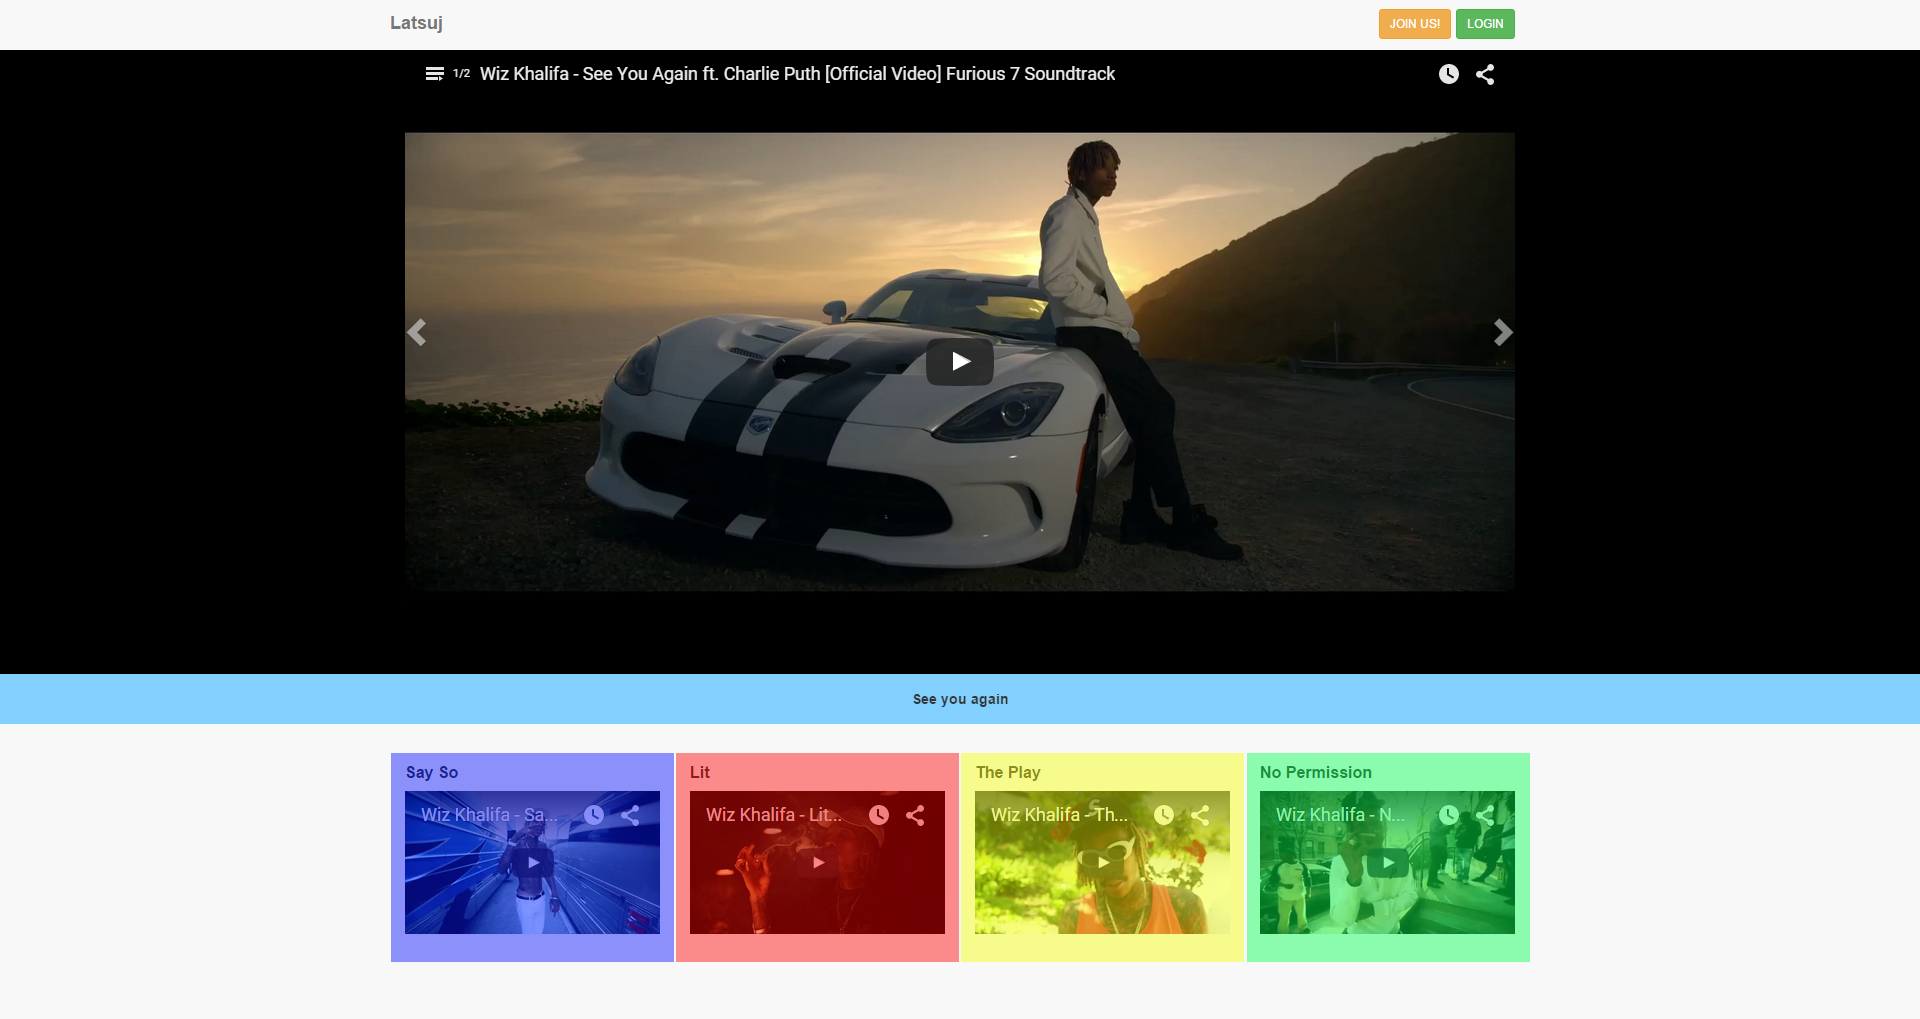
\includegraphics[width=0.48\textwidth]{pc4}
  \end{center}
  \vspace{-20pt}
  \caption{Les 4 blocs}
  \vspace{-10pt}
\end{wrapfigure} 

Ce module permet d'ajouter une nouvelle node HTML nomm\'e \og my-col-25-100 \fg{}. Ce dernier permet de faire la division et le repositionnement des clips musicaux en bas de page. J'ai colori\'e chacun des \'el\'ements utilisant ce module sur la figure 8. Sur cette figure, la dimension de la fen\^etre est sup\'erieur \`a 1500px. Dans le code pr\'ec\'edent, les r\`egles en bleu sont celles actives. On remarque que la taille (\og width \fg{} ) est sp\'ecifi\'e \`a 25\% du container. Chacun des clips prend donc 25\%, ce qui apparait bien sur la figure \`a droite. Ensuite, si l'on r\'eduit la fen\^etre, nous arriverons au point d'ancrage \`a 1500px. Les r\`egles appliqu\'es seront donc celles \'ecrites en bleu puis en rouge. Les r\`egles rouges donneront de nouvelles valeurs aux r\`egles en bleu, elles seront r\'e\'ecrites. Dans notre cas, la longueur maximal que pourra prendre un de nos clips musicaux sera de 50\% du container. Ainsi, lorsque 100\% du container est pris par 2 vide\'eos, les suivantes se placeront en dessous. Maintenant, imaginons que nous continuions \`a r\'eduire la fen\^etre jusqu'au point de rupture \`a 900px, chaque vid\'eos prendra la totalit\'e de la largeur de la fen\^etre. L'image ci-dessous montre le r\'esultat obtenue via ces points de rupture avec les mdoules pr\'ec\'dents :

\begin{center}
\vspace{0.5cm}
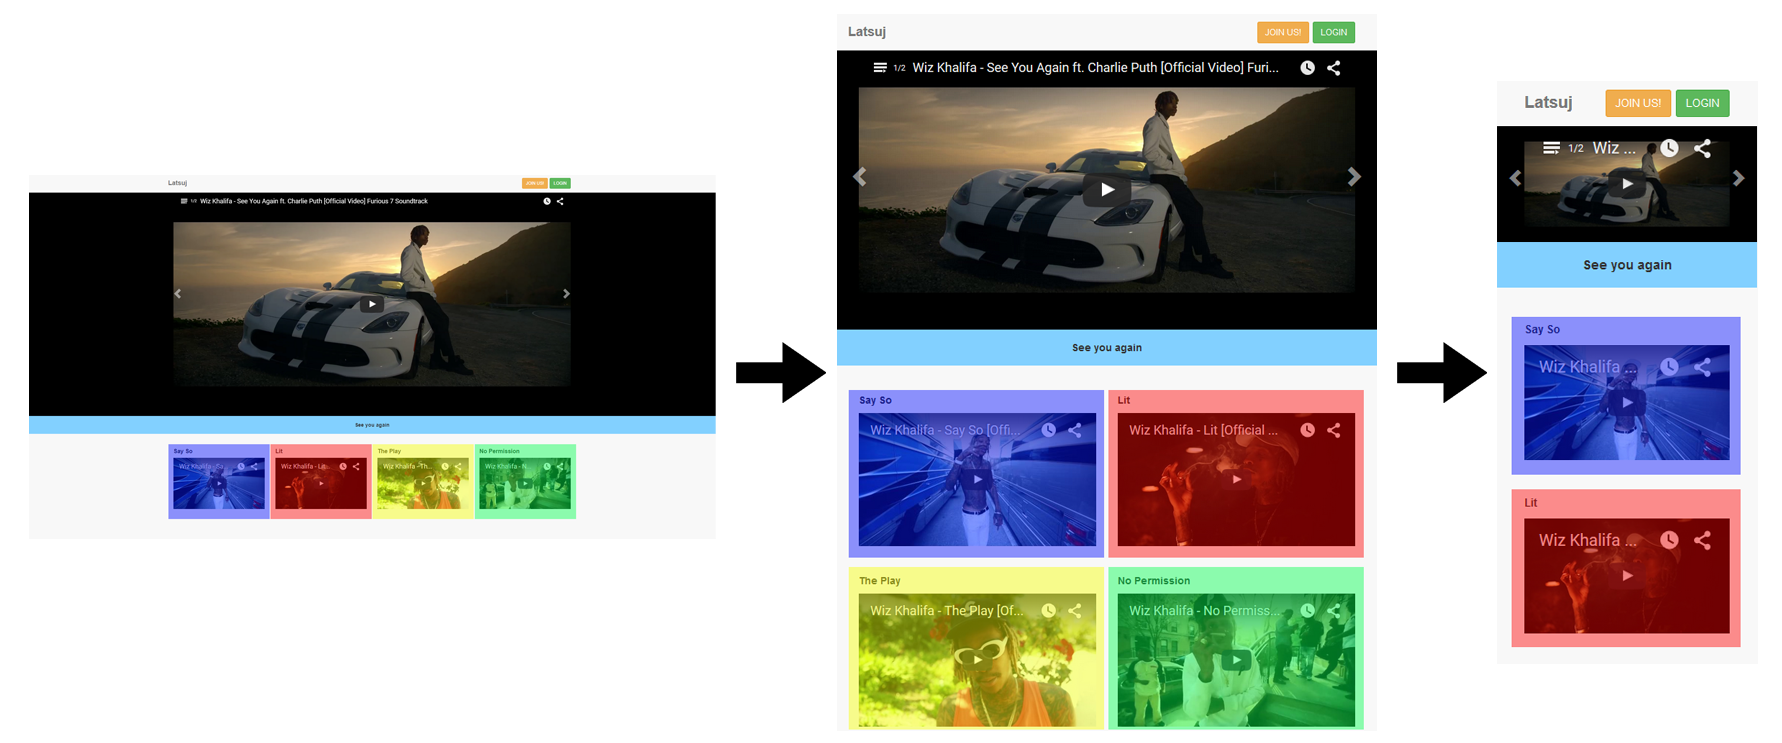
\includegraphics[width=0.8\textwidth]{pc7}
\vspace{0.5cm}\\
\end{center}

\`A travers ces diff\'erents exemples, nous avons pu voir comment faire des points de ruptures sous les deux technologies diff\'erentes. Sur Bootstrap, il est bien plus simple d'utiliser ces points de ruptures. L'utilisation des classes xs, sm, md et lg rendent le principe facile \`a comprendre. Cependant, nous sommes limit\'es par Bootstrap \`a suivre ces quatres points de ruptures. Si le site contient de nombreux autres points de ruptures, Bootstrap perd de sa superbe car cela reviendrait \`a faire du CSS classique. Sur Polymer, il faut bien comprendre les m\'edia queries (points de ruptures) pour pouvoir les utiliser. Comme Polymer fractionne notre code, on se retrouve avec du CSS et donc des points de ruptures qui se retrouvent \'eparpill\'e dans le code. En cas de changement de points de rupture, la maintenance peut vide devenir difficile. 

\subsection{Grille de positionnement}

\begin{wrapfigure}{r}{0.5\textwidth}
  \vspace{-25pt}
  \begin{center}
    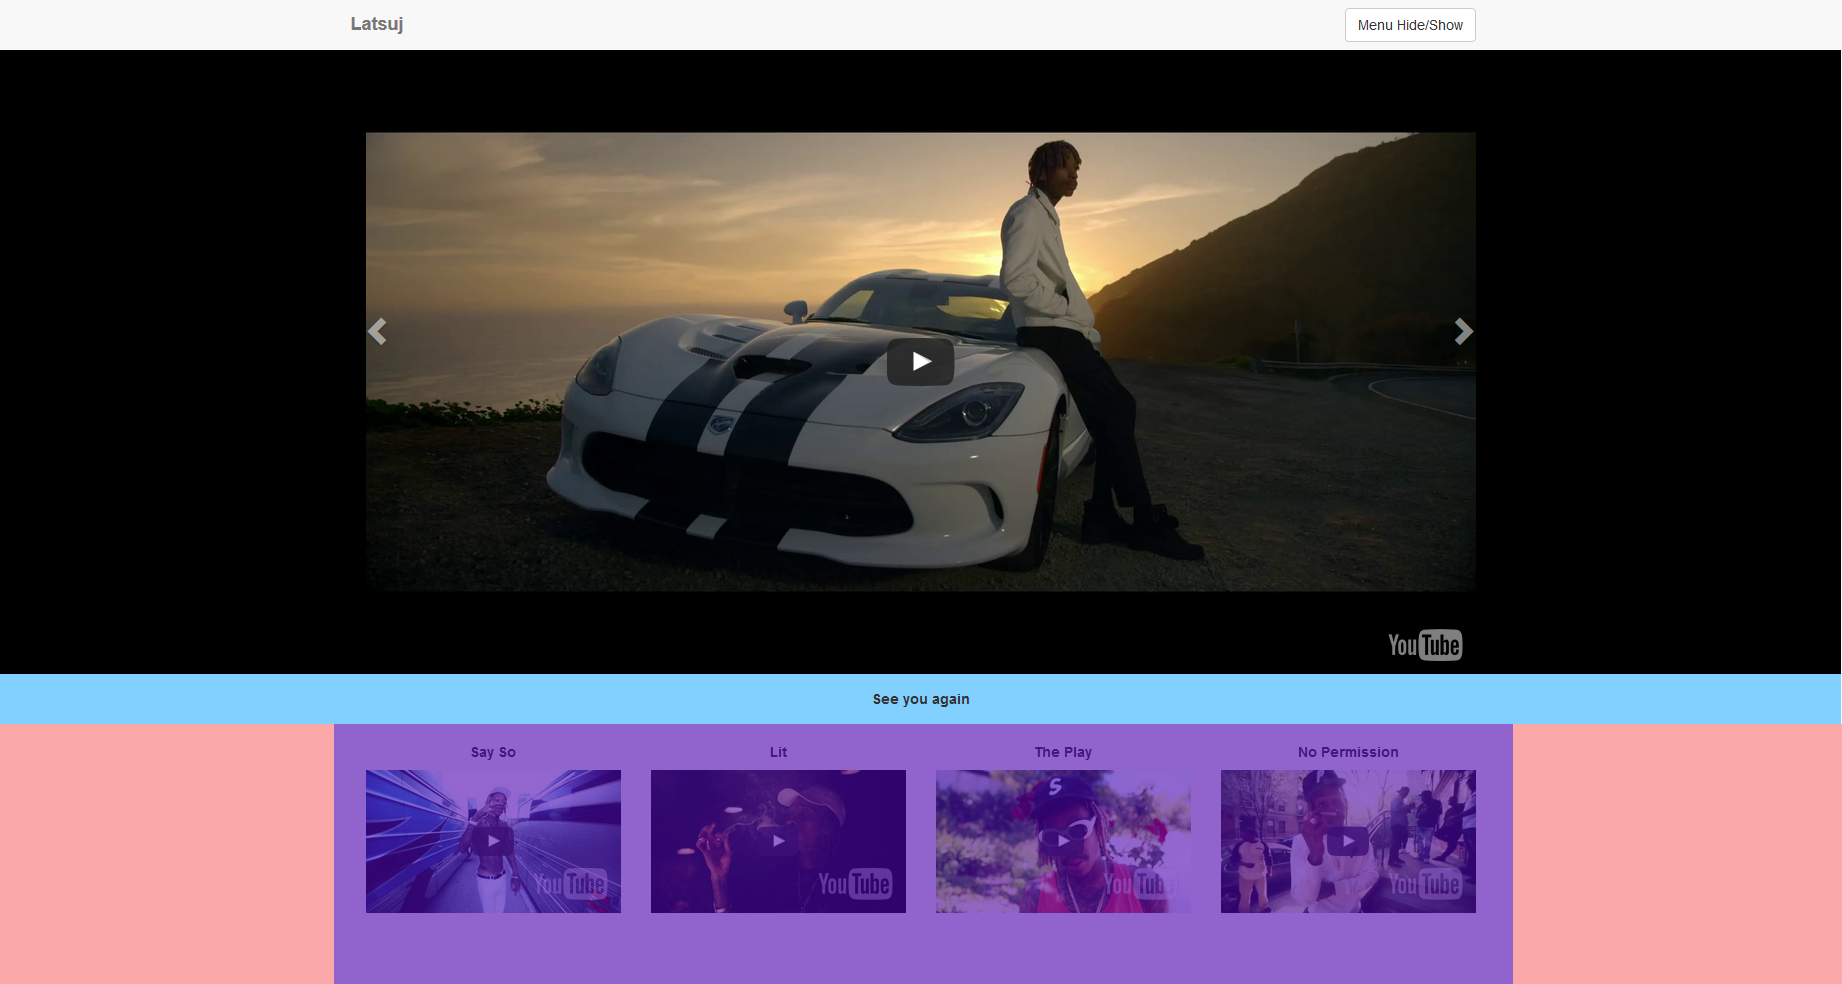
\includegraphics[width=0.48\textwidth]{p10}
  \end{center}
  \vspace{-20pt}
  \caption{Le container du bas de page}
  \vspace{-10pt}
\end{wrapfigure} 

Les grilles de positionnements consiste en un dimensionnement relatif des diff\'erents blocs de la page. J'ai d\'ej\`a partiellement \'evoqu\'e ce point. Je vais essayer de me concentrer ici sur ce point en particulier. Comme dit dans le chapitre pr\'ec\'dent, les grilles se placent dans des containers. Qu'est qu'un container ? Sur la figure 9, j'ai repr\'sent\'e en violet, le container du bas de la page. On peux aussi l'obtenir en analysant le code avec Firebug (F12). Cet espace violet est la place maximale que peux prendre le contenue ici.\\

\begin{wrapfigure}{r}{0.5\textwidth}
  \vspace{-25pt}
  \begin{center}
    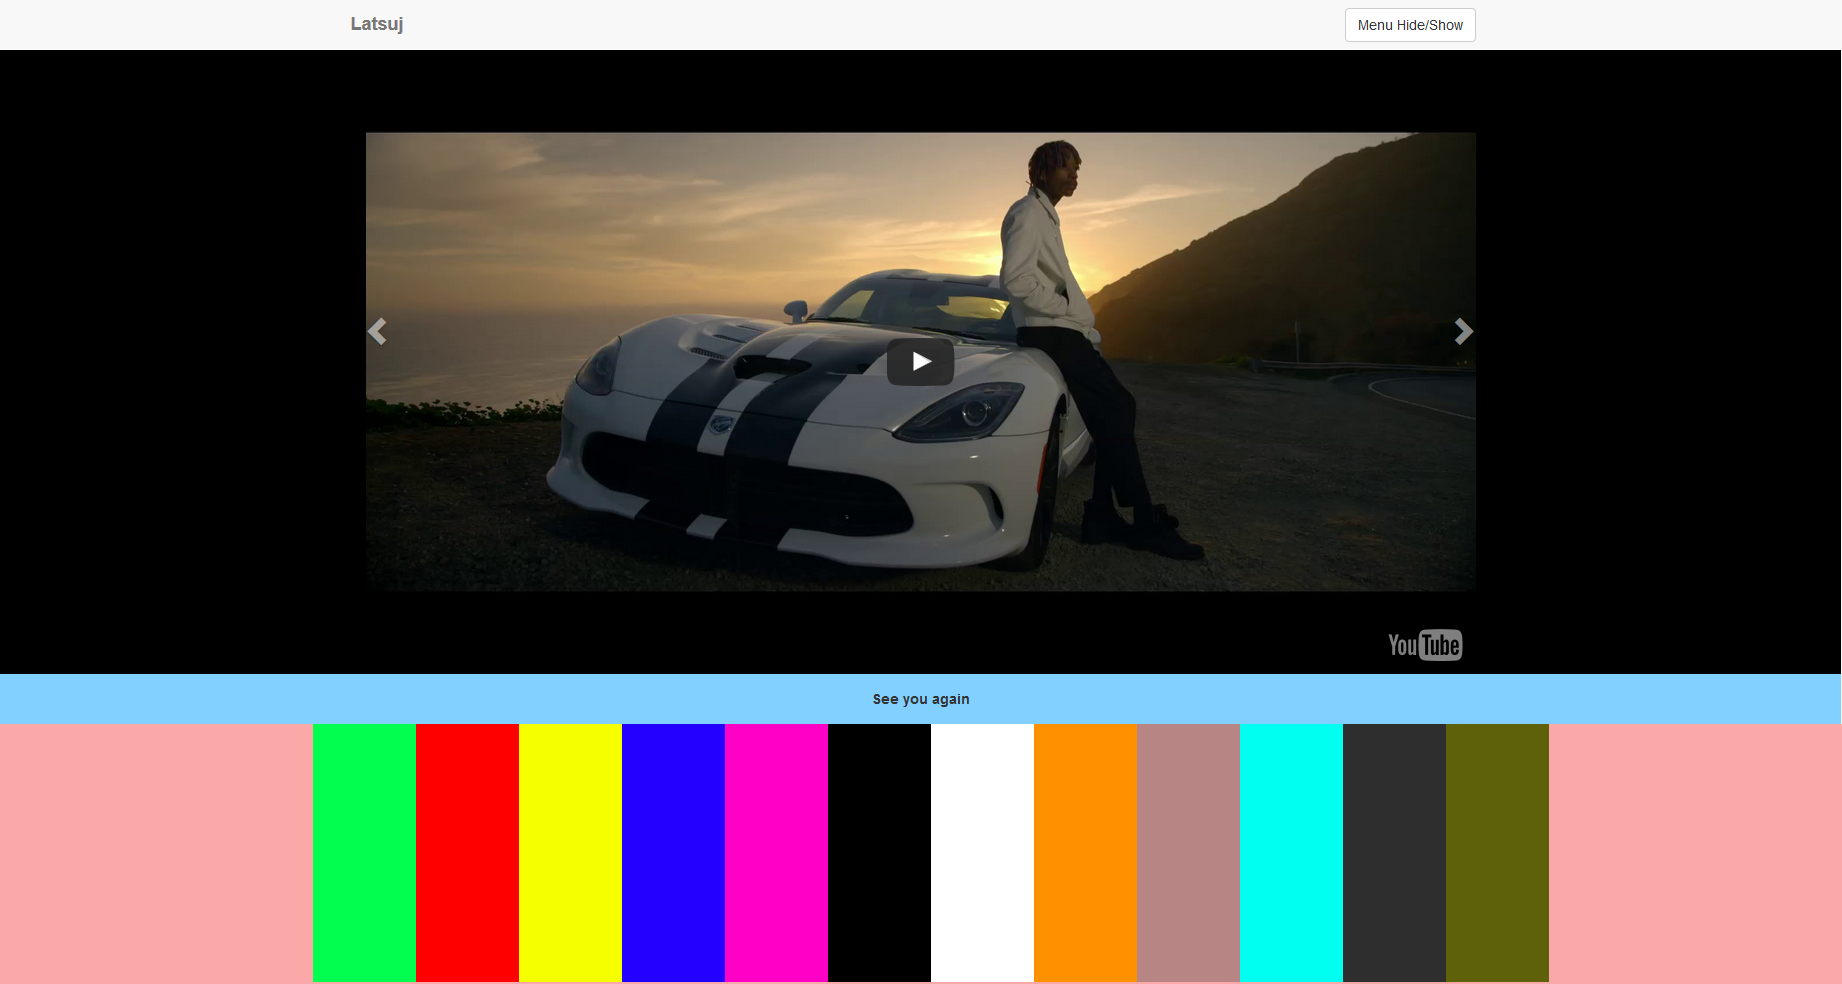
\includegraphics[width=0.48\textwidth]{p12}
  \end{center}
  \vspace{-20pt}
  \caption{Les 12 divisions d'un container}
  \vspace{-10pt}
\end{wrapfigure} 

Lorsque l'on utilise la classe \og row \fg{} dans Bootstrap, on divise ce container en 12 parties \'egales. Avec Polymer, le principe que j'ai d\'evelopp\'e est globalement le m\^eme cependant j'ai d\`u reconstruire ces divisions de A \`a Z via les m\'edia queries et les attributs CSS (en particulier : width). Sur la figure 10, j'ai repr\'esent\'e chacune des divisions d'une couleur diff\'erente. Ensuite, on peux d\'efinir combien de colonnes ou divisions pourra prendre un \'el\'ement. (voir les explication du chapitre pr\'ec\'edent).\\

\begin{wrapfigure}{r}{0.5\textwidth}
  \vspace{-25pt}
  \begin{center}
    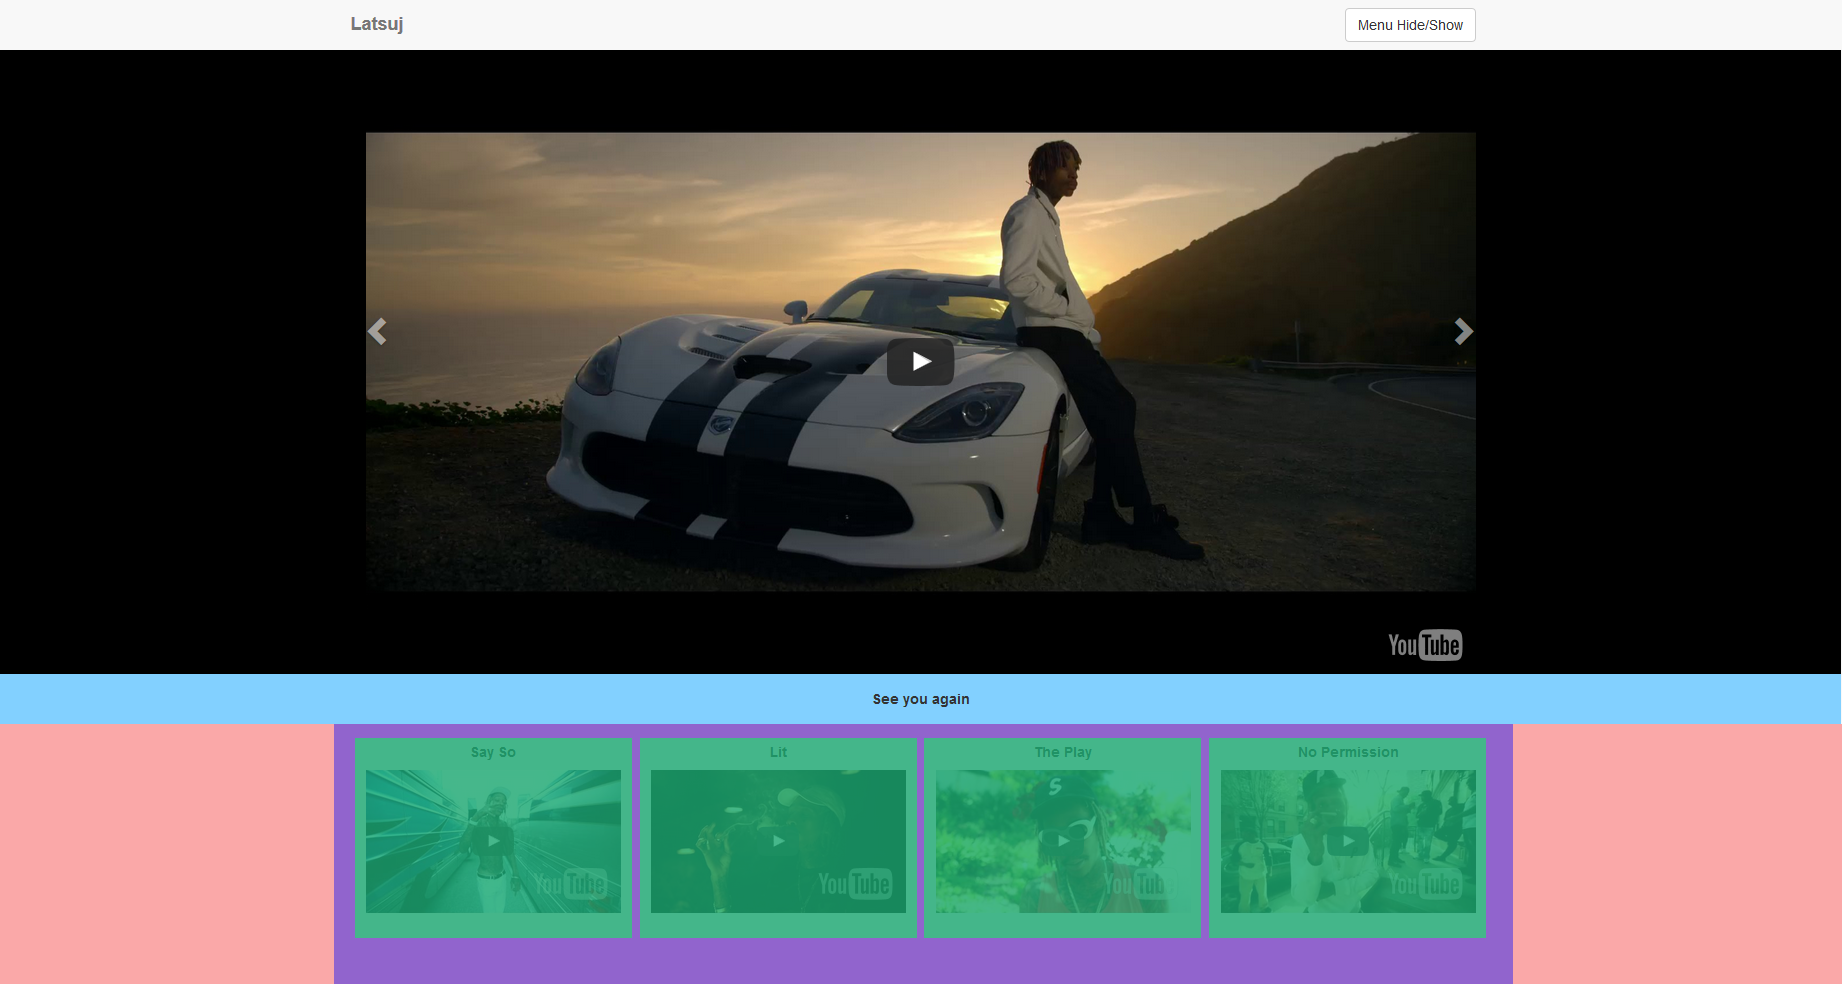
\includegraphics[width=0.48\textwidth]{p11}
  \end{center}
  \vspace{-20pt}
  \caption{Les 12 divisions d'un container}
  \vspace{-10pt}
\end{wrapfigure} 

Pour les clips musicaux en bas de page, j'ai d\'efini pour chacun d'entre eux 3 divisions. Sur Bootstrap, cela se traduit par \og col-XX-3 \fg{} o\`u XX repr\'esente tout simplement les points de rupture que j'ai \'evoqu\'e dans le chapitre pr\'ec\'edent. Avec Polymer, pour r\'ealiser cela, il faut imbriqu\'e deux modules ou balises l'une dans l'autre. La premi\`ere servira de container pour r\'ealiser la m\^eme chose que sur la figure 9 tandis que la deuxi\`eme servira a r\'ealiser les divisions comme sur l'image de droite.\\

Le point important est que les \'el\'ements des grilles sont d\'efinis comme \og float:left \fg{} que ce soit sur Bootstrap ou sur Polymer. Ce qui veut dire qu'un \'el\'ement, ce positionnera toujours le plus \`a gauche possible sur la m\^eme ligne si il y a la place disponible, sinon l'\'el\'ement se positionnera sur une nouvelle ligne. De m\^eme, il y a toujours 12 colonnes sur une ligne peux importe la taille de la fen\^etre. Si jamais les \'el\'ements \'ex\'edent le nombre de colonnes disponibles sur la ligne, il se place automatiquement sur la ligne en dessous.\\

\begin{center}
\vspace{0.5cm}
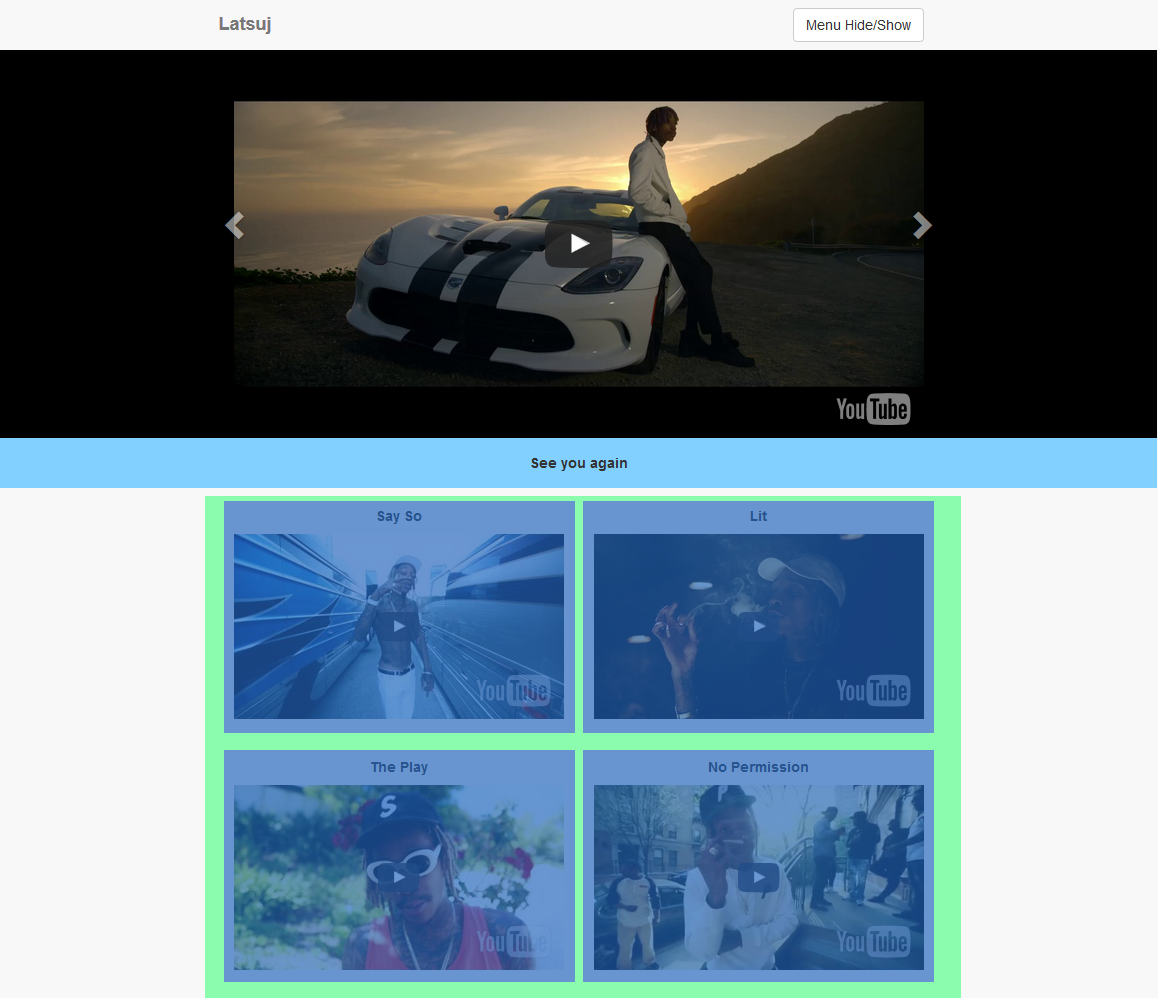
\includegraphics[width=0.8\textwidth]{p13}
\vspace{0.5cm}\\
\end{center}

Comme vue dans les exemples pr\'ec\'edent, les clips musicaux du bas de la page \'etaient affich\'e sur 1 ligne. Sur Bootstrap, cela \'equivaut \`a utiliser la classe \og col-XX-3 \fg{}. Il y a 4 vid\'eos qui utilisent chacune 3 divisions. Sur Polymer, on pr\'ecisera que le bloc utilise 25\% du container en CSS avec l'attribut \og width \fg{}. Maintenant sur l'image ci-dessus, il y a deux lignes. Chacune utilise un syst\`eme de 12 colonnes. La diff\'erence r\'eside simplement dans le nombre de colonne qu'on a permis \`a l'\'el\'ement d'utiliser. Ici, j'ai utilis\'e la classe \og col-XX-6 \fg{} sur Bootstrap. Pour indiquer que chaque vid\'eo prendrait 6 colonnes. Comme il y a 4 clips, les deux premieres vid\'eos ont remplit la premi\`ere ligne puis la troisi\`eme vid\'eo est automatiquement pass\'e \`a la ligne en dessous pour compl\'eter le container.\\

Ainsi, nous avons une id\'ee g\'en\'erale des moyens que j'ai utilis\'e pour faire mon site ainsi qu'une compr\'ehension pouss\'e des techniques que je vais employ\'e pour comprendre comment j'ai form\'e mon site.

\newpage
\section{L'exemple de A \`a Z}

\subsection{Installation}
Installation ?
\subsection{Creation des containers}

Il est maintenant temps de commencer l'application de ce que nous avons vu pr\'ec\'edent dans un exemple concret. Nous allons reproduire l'ensemble de mon site sous les deux technologies que sont Polymer et Bootstrap. Si vous avez compris ce que j'ai expliqu\'e dans le chapitre suivant, il faut commencer par cr\'eer nos container. C'est \`a dire nos \'el\'ements qui serviront de base \`a nos grilles de positionnement.\\

\begin{wrapfigure}{r}{0.5\textwidth}
  \vspace{-25pt}
  \begin{center}
    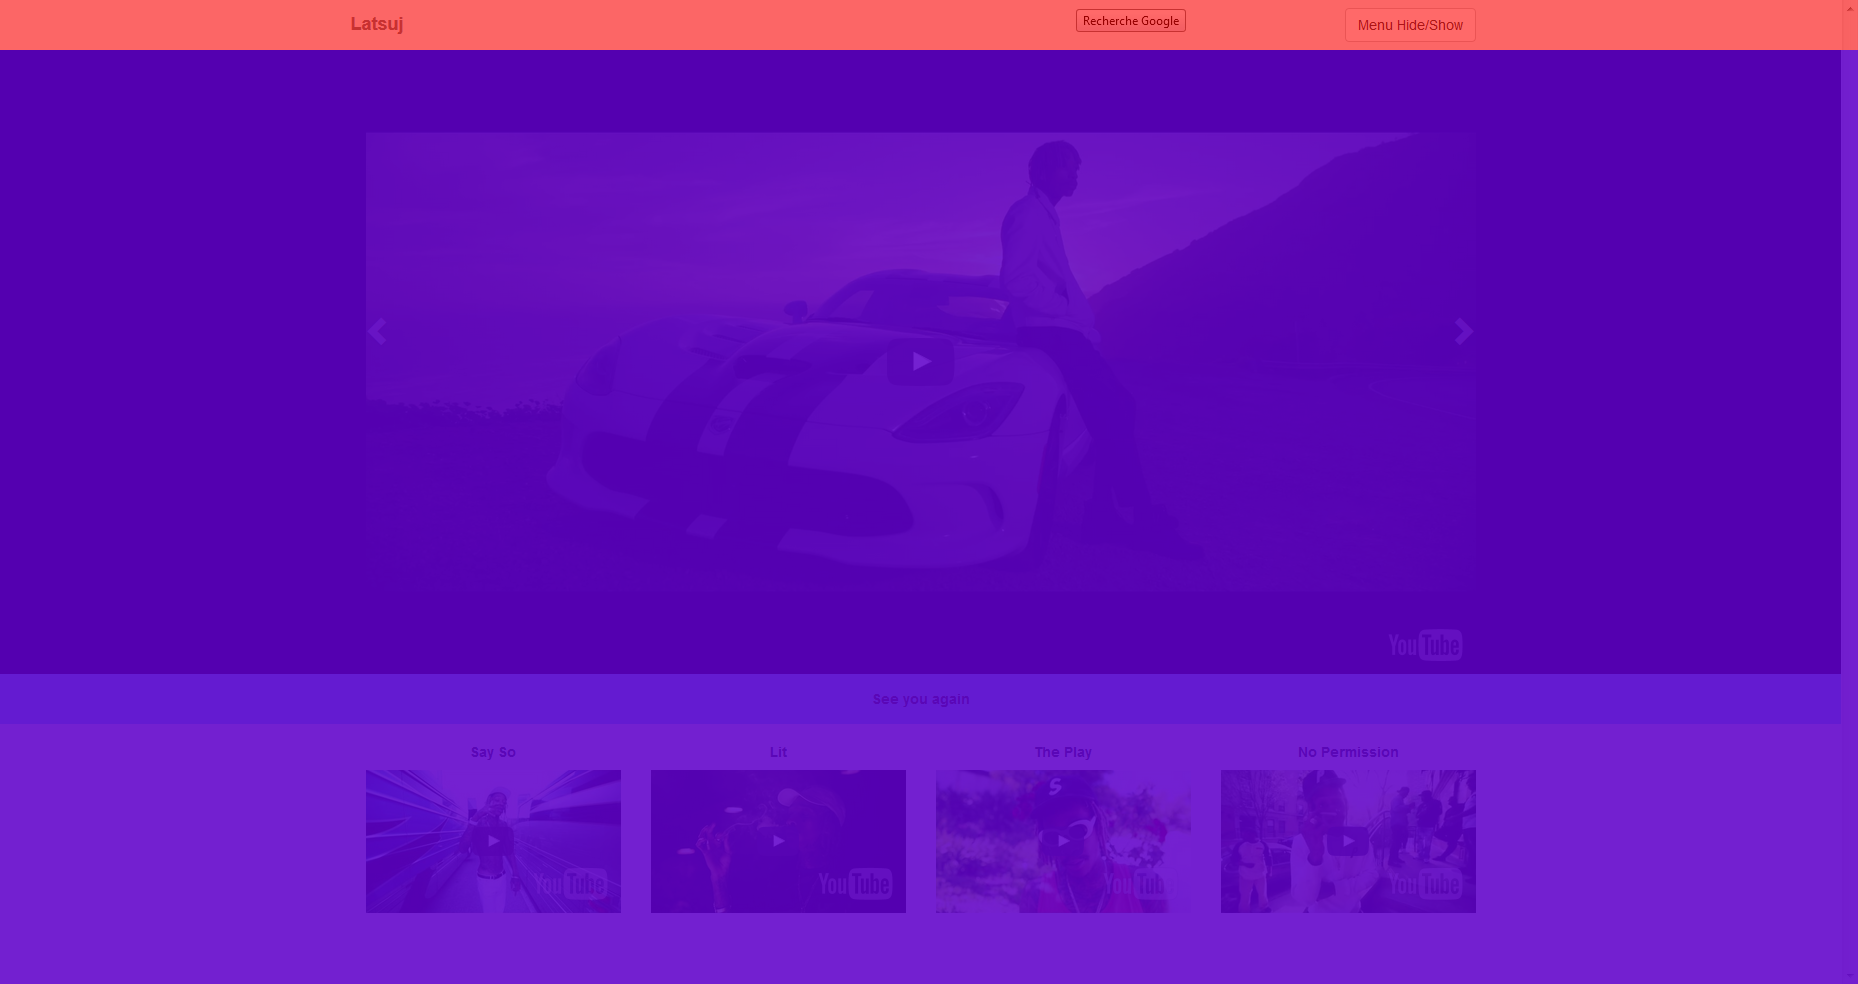
\includegraphics[width=0.48\textwidth]{p18}
  \end{center}
  \vspace{-20pt}
  \caption{Les 12 divisions d'un container}
  \vspace{-10pt}
\end{wrapfigure} 

Sur mon exemple, il y a deux grands blocs principaux. Un container ou plutot une barre principale qui se trouve en haut du site (couleur rouge sur l'image \`a droite) et une partie contenue qui est en fait un grand carousel (couleur violette sur l'image \`a droite). La partie violette sera une partie du site qui sera anim\'e via un script JQuery mais suivra globalement la m\^eme structure.\\

Sous Bootstrap, j'ai utilis\' trois classes sur des balises HTML pour r\'ealiser cela facilement : \og container-fluid \fg{}, \og navbar \fg{} et \og container \fg{}. La premi\`ere permet de sp\'ecifi\'e que nous utiliserons 100\% de la largeur de la fen\^etre. La seconde est la balise pour sp\'ecifi\'e o\`u se trouve notre menu de navigation. La derni\`ere permet de prendre la dimension en pixel avant le point de rupture. Les autres classes qui se trouvent dans l'exemple ci-dessous ne sont que des classes am\'eliorant le design et ne sont donc pas n\'ec\'essaire pour reproduire mon exemple. Ainsi je n'expliquerais pas leurs utilit\'e, la plupart \'etant expliqu\'e dans la documentation de Bootstrap. 
\vspace{0.5cm}\\
\fbox{\parbox{\textwidth}{
...\\
<body>\\
\hspace*{0.6cm}<nav class="navbar navbar-default navbar-static-top">\\
\hspace*{1.2cm}<div class="container-fluid black">\\
\hspace*{1.2cm}</div>\\
\hspace*{0.6cm}</nav>\\
\hspace*{0.6cm}<div class="container-fluid black">\\
\hspace*{0.6cm}</div>\\
</body>\\
...
}}
\vspace{0.5cm}\\
Sous Polymer, nous allons simplement reproduire le comportement des classes pr\'ec\'edentes et en faire de nouveaux \'el\'ements   du DOM (Document Object Model). Pour faire cela proprement, j'ai utilis\'e Firebugs et est analys\'e le CSS utilis\'e sur Bootstrap pour reproduire le style de ces classes. Le code sous Polymer dans la page index est le suivant :
\vspace{0.5cm}\\
\fbox{\parbox{\textwidth}{
...\\
<body>\\
\hspace*{0.6cm}<bar-top>\\
\hspace*{1.2cm}<my-container>\\
\hspace*{1.2cm}</my-container>\\
\hspace*{0.6cm}</bar-top>\\
\hspace*{0.6cm}<my-container-full>\\
\hspace*{0.6cm}</my-container-full>\\
</body>\\
...
}}
\vspace{0.5cm}\\
Pour que ce code fonctionne correctement, il faut bien \'evidemment cr\'eer les modules. Un module est simplement une page HTML avec une certaine syntaxe que nous incorporons dans la page principale (index.html) avec le code suivant \`a placer entre les balises HEAD :
\vspace{0.5cm}\\
\fbox{\parbox{\textwidth}{
<link rel="import" href="bar-top.html">\\
<link rel="import" href="my-container.html">\\
<link rel="import" href="my-container-full.html">
}}
\vspace{0.5cm}\\

Le fichier bar-top.html qui repr\'esentera notre nouveau \'el\'ement du DOM aura son style CSS fix\'e \`a lui. \`A noter que la syntaxe est extr\^emement importante. Un module doit obligatoirement \^etre nomm\'e de la fa\c{c}on suivante (xxxx-xxxx). Le code ci-dessous est \`a ajouter au m\^eme niveau que index.html dans le fichier \textbf{bar-top.html} :
\vspace{0.5cm}\\
\fbox{\parbox{\textwidth}{
<dom-module id="bar-top">\\
\hspace*{0.6cm}<template>\\
\hspace*{1.2cm}<style>\\
\hspace*{1.8cm}\color{red}{:host} \{	\\		
\hspace*{2.4cm}\color{black}{background-color: \#f8f8f8;\\
\hspace*{2.4cm}border-color: \#e7e7e7;\\
\hspace*{2.4cm}z-index: 1000;\\
\hspace*{2.4cm}border-width: 0 0 1px;\\
\hspace*{2.4cm}position: relative;\\
\hspace*{2.4cm}min-height: 50px;\\
\hspace*{2.4cm}display: block;\\
\hspace*{2.4cm}box-sizing: border-box;\\		
\hspace*{2.4cm}border: none;\\
\hspace*{1.8cm}\}		\\		
\hspace*{1.8cm}@media (min-width: 768px) \{\\
\hspace*{2.4cm}:host \{\\
\hspace*{3.0cm}border-radius: 0;\\
\hspace*{2.4cm}\}	\\	
\hspace*{1.8cm}\}\\
\hspace*{1.2cm}</style>}\\
\hspace*{1.2cm}\color{red}{<content></content>}\\		
\hspace*{0.6cm}\color{black}{</template>\\
\hspace*{0.6cm}<script>}\\
\hspace*{0.6cm}\color{red}{Polymer(\{\\
\hspace*{1.2cm}is: "bar-top"\\
\hspace*{0.6cm}\});}\\
\hspace*{0.6cm}\color{black}{</script>\\
</dom-module>}
}}
\vspace{0.5cm}\\
Comme dit plus haut, il s'agit du module \og bar-top \fg{}, le lien avec ce code est r\'ealiser avec l'id du dom-module ainsi que le script qui sp\'ecifie son nom. \og :host \fg{} repr\'esente le module lui-m\^eme. Tous les r\`egles CSS inscritent dans ce tag prendra automatiquement effet pour tout \'el\'ement <bar-top></bar-top>. Enfin la balise \og content \fg{} est le point d'ancrage du nouvelle \'el\'ement. C'est \`a dire que le code se trouvant entre les balises <bar-top> et </bar-top> se positionnera \`a l'int\'erieur des balises \og content \fg{}. Pour les m\'edia queries, j'ai d\'ej\`a expliqu\'e leurs fonctionnements dans le chapitre pr\'ec\'edent.\\
Ainsi la cr\'eation de module prendra toujours la m\^eme forme, il faut reproduire l'op\'eration pour que les deux autres modules prennent eux aussi effet :   
\vspace{0.5cm}\\
\fbox{\parbox{\textwidth}{
<dom-module id="my-container">\\
\hspace*{0.6cm}<template>\\
\hspace*{1.2cm}<style>\\
\hspace*{1.8cm}:host \{\\
\hspace*{2.4cm}padding-right: 15px;\\
\hspace*{2.4cm}padding-left: 15px;\\
\hspace*{2.4cm}margin-right: auto;\\
\hspace*{2.4cm}margin-left: auto;\\
\hspace*{2.4cm}box-sizing: border-box;\\
\hspace*{2.4cm}display: block;\\
\hspace*{2.4cm}height: auto;\\
\hspace*{1.8cm}\}\\	
\hspace*{1.8cm}@media (min-width:900px) \{\\
\hspace*{2.4cm}:host \{\\
\hspace*{3.0cm}width:700px;\\
\hspace*{2.4cm}\}\\
\hspace*{1.8cm}\}\\
\hspace*{1.8cm}@media (min-width:1200px) \{\\
\hspace*{2.4cm}:host \{\\
\hspace*{3.0cm}width:970px;\\
\hspace*{2.4cm}\}\\
\hspace*{1.8cm}\}\\
\hspace*{1.8cm}@media (min-width:1500px) \{\\
\hspace*{2.4cm}:host \{\\
\hspace*{3.0cm}width:1170px;\\
\hspace*{2.4cm}\}\\
\hspace*{1.8cm}\}\\
\hspace*{1.2cm}</style>\\
\hspace*{1.2cm}<content></content>\\
\hspace*{0.6cm}</template>\\
\hspace*{0.6cm}<script>\\
\hspace*{0.6cm}Polymer(\{\\
\hspace*{1.2cm}is: "my-container"\\
\hspace*{0.6cm}\});\\
\hspace*{0.6cm}</script>\\
</dom-module>
}}
\vspace{0.5cm}\\
\fbox{\parbox{\textwidth}{
<dom-module id="my-container-full">\\
\hspace*{0.6cm}<template>\\
\hspace*{1.2cm}<style>	\\	
\hspace*{1.8cm}:host \{\\	
\hspace*{2.4cm}display: block;	\\
\hspace*{2.4cm}position: absolute;\\
\hspace*{2.4cm}width: 100\%;\\
\hspace*{2.4cm}height: auto;\\
\hspace*{1.8cm}\}\\
\hspace*{1.2cm}</style>\\
\hspace*{1.2cm}<content></content>\\
\hspace*{0.6cm}</template>\\
\hspace*{0.6cm}<script>\\
\hspace*{0.6cm}Polymer(\{\\
\hspace*{1.2cm}is: "my-container-full"\\
\hspace*{0.6cm}\});\\
\hspace*{0.6cm}</script>\\
</dom-module>
}}
\vspace{0.5cm}\\
Ainsi nous obtenons le m\^eme r\'esultat avec les deux technologies. Nos containers \'etant maintenant pr\^et, nous allons nous occup\'e de la barre du haut (zone rouge dans la figure 12).

\subsection{Barre de menu}

\begin{center}
\vspace{0.5cm}

\includegraphics[width=\textwidth]{p19}
\end{center}

Le menu est compos\'e de ma signature \og Latsuj \fg{}, tout simplement mon nom \`a l'envers ainsi qu'un bouton pour afficher ou cacher le menu. J'ai choisi de mettre ma signature \`a gauche \`a cause de la nature de l'utilisateur. Un humain lit toujours de mani`ere inconsciente en diagonale. C'est aussi ce que l'on nomme lecture-rapide. Le premier mot que l'utilisateur verra sera donc ma signature. Ensuite, j'ai mis le bouton \`a droite pour faire echo au texte \`a gauche, la nature pr\'ef\`ere ce qui est sym\'etrique, ainsi que pour utiliser toutes la place disponible. Sous Bootstrap, comme toujours nous avons des classes pour r\'ealiser cela sans trop se fatiguer. Par rapport \`a ce dont j'ai parl\'e pr\'ec\'edemment, il y aura 3 nouvelles classes ici que je n'ai pas encore \'evoqu\'e : \og pull-left \fg{},\og pull-right \fg{}, \og btn \fg{}. Les deux classes \og pull \fg{} permettent de pousser leurs contenues vers la gauche ou la droite. \og btn \fg{} permet quant \`a elle de mettre le style d'un bouton sur le composant o\`u on l'utilise. On obtient alors notre menu assez facilement :
\vspace{0.5cm}\\
\fbox{\parbox{\textwidth}{
\hspace*{0.6cm}<nav class="navbar navbar-default navbar-static-top">\\
\hspace*{1.2cm}<div class="container"> 	\\
\hspace*{1.8cm}<div class="row">\\   
\hspace*{2.4cm}<div class="col-sm-12 col-md-12 col-lg-12">\\
\hspace*{3.0cm}<div class="pull-left">\\
\hspace*{3.6cm}<strong class="navbar-brand">Latsuj</strong>\\
\hspace*{3.0cm}</div>\\
\hspace*{3.0cm}<div class="pull-right navbar-brand">\\
\hspace*{3.6cm}<div class="menu-toggle btn btn-default">Menu Hide/Show</div>\\
\hspace*{3.0cm}</div>\\
\hspace*{2.4cm}</div>\\
\hspace*{1.8cm}</div>\\
\hspace*{1.2cm}</div>\\
\hspace*{0.6cm}</nav>
}}
\vspace{0.5cm}\\
A noter ici que nous aurions pu sp\'ecifier que notre signature prenne 2 colonnes, que le bouton en prenne aussi 2 colonnes et mettre un offset entre les deux de 8 colonnes. Cependant, j'ai pr\'ef\'er\'e cette m\'ethode car cela me fait moins de ligne de code donc un code plus clair. Les classes dont je n'explique pas le r\^ole ne sont l\`a que pour rendre les choses plus jolie et ne sont pas n\'eccesaire pour reproduire l'architecture de mon site/exemple. Avec le simple exemple, ci-dessus, nous obtenons sous Bootstrap notre menu. Sous Polymer, il va falloir comme pr\'ec\'edemment reproduire le comportement des blocs de Bootstrap en cr\'eant de nouvelles nodes. Dans le code qui va suivre, il n'y a rien de nouveau, ni de compliqu\'e, ce n'est que du CSS :
\vspace{0.5cm}\\
\fbox{\parbox{\textwidth}{
<dom-module id="my-row">\\
\hspace*{0.6cm}<template>\\
\hspace*{1.2cm}<style>	\\	
\hspace*{1.8cm}:host \{\\
\hspace*{2.4cm}display: block;\\
\hspace*{2.4cm}position: relative;\\
\hspace*{2.4cm}margin-right: -15px;\\
\hspace*{2.4cm}margin-left: -15px;\\
\hspace*{2.4cm}box-sizing: border-box;\\
\hspace*{1.8cm}\}\\
\hspace*{1.2cm}</style>\\
\hspace*{1.2cm}<content></content>\\
\hspace*{0.6cm}</template>\\
\hspace*{0.6cm}<script>\\
\hspace*{1.2cm}Polymer(\{\\
\hspace*{1.8cm}is: "my-row"\\
\hspace*{1.2cm}\});\\
\hspace*{0.6cm}</script>\\
</dom-module>
}}
\vspace{0.5cm}

Il n'y a rien de particulier sur ce module \og my-row \fg{} qui reproduit le comportement de la classe \og row \fg{} de Boostrap. Notons cependant que dans Polymer, les nouveaux modules sont toujours sp\'ecifi\'e comme \og display:inline \fg{}, il faut donc tr\`es souvent les passer en \og display:bloc \fg{}. Notons par ailleurs l'utilisation de box-sizing qui n'est peut-\^etre pas n\'ecessaire ici. Ayant voulu cr\'e\'e un site fonctionnant sur tout les navigateurs, cet attribut est essentiel. Cependant, Polymer \'etant tr\`es mal support\'e pour l'instant, cet attribut perd de son int\'eret au jour d'aujourd'hui. Si les navigateurs s'effor\c{c}aient de faire le n\'ecessaire pour supporter Polymer, il n'y aurait pas besoin de modifier mon exemple car j'aurais d\'ej\`a pr\'evu cela.
\vspace{0.5cm}\\
\fbox{\parbox{\textwidth}{
<dom-module id="col-top">\\
\hspace*{0.6cm}<template>\\
\hspace*{1.2cm}<style>\\
\hspace*{1.8cm}:host \{\\
\hspace*{2.4cm}display: block;\\
\hspace*{2.4cm}position: relative;\\
\hspace*{2.4cm}padding-right: 15px;\\
\hspace*{2.4cm}padding-left: 15px;\\
\hspace*{2.4cm}box-sizing: border-box;\\
\hspace*{2.4cm}height: 50px; \\  
\hspace*{2.4cm}float: left;\\
\hspace*{2.4cm}width: 100\%;\\
\hspace*{1.8cm}\}\\
\hspace*{1.8cm}</style>\\
\hspace*{1.8cm}<content></content>\\
\hspace*{1.2cm}</template>\\
\hspace*{1.2cm}<script>\\
\hspace*{1.2cm}Polymer(\{\\
\hspace*{1.8cm}is: "col-top"\\
\hspace*{1.2cm}\});\\
\hspace*{0.6cm}</script>\\
</dom-module>
}}
\vspace{0.5cm}
d
\vspace{0.5cm}\\
\fbox{\parbox{\textwidth}{
<dom-module id="pull-left">\\
\hspace*{0.6cm}<template>\\
\hspace*{1.2cm}<style>\\
\hspace*{1.8cm}:host \{\\
\hspace*{2.4cm}display: block;\\
\hspace*{2.4cm}float: left!important;\\
\hspace*{2.4cm}box-sizing: border-box;\\
\hspace*{2.4cm}margin-left: -15px;\\  		
\hspace*{2.4cm}height: 50px;\\
\hspace*{2.4cm}padding: 15px 15px;\\
\hspace*{2.4cm}font-size: 18px;\\
\hspace*{2.4cm}line-height: 40px;\\
\hspace*{2.4cm}margin-top: -15px;\\
\hspace*{1.8cm}\}\\
\hspace*{1.8cm}</style>	\\
\hspace*{1.8cm}<content></content> 	\\
\hspace*{1.2cm}</template>\\
\hspace*{1.2cm}<script>\\
\hspace*{1.2cm}Polymer(\{\\
\hspace*{1.8cm}is: "pull-left"\\
\hspace*{1.2cm}\});\\
\hspace*{0.6cm}</script>\\
</dom-module>
}}
\vspace{0.5cm}
 d
\vspace{0.5cm}\\
\fbox{\parbox{\textwidth}{
<dom-module id="pull-right">\\
\hspace*{0.6cm}<template>\\
\hspace*{1.2cm}<style>\\
\hspace*{1.8cm}:host \{\\
\hspace*{2.4cm}display: block;\\
\hspace*{2.4cm}float: right!important;\\
\hspace*{2.4cm}box-sizing: border-box;\\
\hspace*{2.4cm}margin-left: -15px;\\  		
\hspace*{2.4cm}height: 50px;\\
\hspace*{2.4cm}padding: 15px 15px;\\
\hspace*{2.4cm}font-size: 18px;\\
\hspace*{2.4cm}line-height: 40px;\\
\hspace*{2.4cm}margin-top: -15px;\\
\hspace*{1.8cm}\}\\
\hspace*{1.8cm}</style>	\\
\hspace*{1.8cm}<content></content> 	\\
\hspace*{1.2cm}</template>\\
\hspace*{1.2cm}<script>\\
\hspace*{1.2cm}Polymer(\{\\
\hspace*{1.8cm}is: "pull-right"\\
\hspace*{1.2cm}\});\\
\hspace*{0.6cm}</script>\\
</dom-module>
}}
\vspace{0.5cm} 
  
 d
\vspace{0.5cm}\\
\fbox{\parbox{\textwidth}{
<dom-module id="title-top">\\
\hspace*{0.6cm}<template>\\
\hspace*{1.2cm}<style>\\
\hspace*{1.8cm}:host \{ \\   
\hspace*{2.4cm}margin-left:-15px;\\
\hspace*{2.4cm}line-height: 40px;\\
\hspace*{2.4cm}float: left;\\
\hspace*{2.4cm}height: 50px;\\
\hspace*{2.4cm}padding: 15px 15px;\\
\hspace*{2.4cm}font-size: 18px;\\
\hspace*{2.4cm}margin-top: -12px;	\\	
\hspace*{2.4cm}color:\#777;\\
\hspace*{1.8cm}\}	  	\\			  	
\hspace*{1.8cm}b,strong \{\\
\hspace*{2.4cm}font-weight:700;\\
\hspace*{1.8cm}\}\\
\hspace*{1.2cm}</style>\\
\hspace*{1.8cm}<strong>Latsuj</strong>\\ 	
\hspace*{1.2cm}</template>\\
\hspace*{1.2cm}<script>\\
\hspace*{1.2cm}Polymer(\{\\
\hspace*{1.8cm}is: "title-top"\\
\hspace*{1.2cm}\});\\
\hspace*{0.6cm}</script>\\
</dom-module>
}}
\vspace{0.5cm} 

 d
\vspace{0.5cm}\\
\fbox{\parbox{\textwidth}{
<dom-module id="my-button">
\hspace*{0.6cm}<template>\\
\hspace*{1.2cm}<style>	\\	
\hspace*{1.8cm}:host \{	\\
\hspace*{2.4cm}color: \#333;\\
\hspace*{2.4cm}background-color: \#FFF;\\
\hspace*{2.4cm}display: inline-block;\\
\hspace*{2.4cm}margin-bottom: 0px;\\
\hspace*{2.4cm}font-weight: normal;\\
\hspace*{2.4cm}text-align: center;\\
\hspace*{2.4cm}vertical-align: middle;\\
\hspace*{2.4cm}cursor: pointer;\\
\hspace*{2.4cm}background-image: none;\\
\hspace*{2.4cm}border: 1px solid \#CCC;\\
\hspace*{2.4cm}white-space: nowrap;\\
\hspace*{2.4cm}padding: 6px 12px;\\
\hspace*{2.4cm}font-size: 14px;\\
\hspace*{2.4cm}line-height: 1.42857;\\
\hspace*{2.4cm}border-radius: 4px;\\
\hspace*{2.4cm}-moz-user-select: none;\\
\hspace*{2.4cm}box-sizing: border-box;\\
\hspace*{1.8cm}\}\\
\hspace*{1.8cm}:host(:focus)\{\\
\hspace*{2.4cm}color: \#333;\\
\hspace*{2.4cm}background-color: \#E6E6E6;\\
\hspace*{2.4cm}border-color: \#8C8C8C;	\\	
\hspace*{1.8cm}\}	\\	
\hspace*{1.8cm}:host(:active) \{\\
\hspace*{2.4cm}color: \#333;\\
\hspace*{2.4cm}background-color: \#D4D4D4;\\
\hspace*{2.4cm}border-color: \#8C8C8C;\\
\hspace*{2.4cm}outline: 0px none;\\
\hspace*{2.4cm}background-image: none;\\
\hspace*{2.4cm}box-shadow: 0px 3px 5px rgba(0, 0, 0, 0.125) inset;\\
\hspace*{1.8cm}\}\\
\hspace*{1.2cm}</style>\\
\hspace*{1.8cm}<div>Menu Hide/Show</div>\\
\hspace*{1.2cm}</template>\\
\hspace*{1.2cm}<script>\\
\hspace*{1.2cm}Polymer(\{\\
\hspace*{1.8cm}is: "my-button"\\
\hspace*{1.2cm}\});\\
\hspace*{0.6cm}</script>\\
</dom-module>
}}
\vspace{0.5cm} 

\newpage
\section{Bootstrap ou Polymer}

\subsection{Compatibilit\'e}

\begin{wrapfigure}{r}{0.5\textwidth}
  \vspace{-25pt}
  \begin{center}
    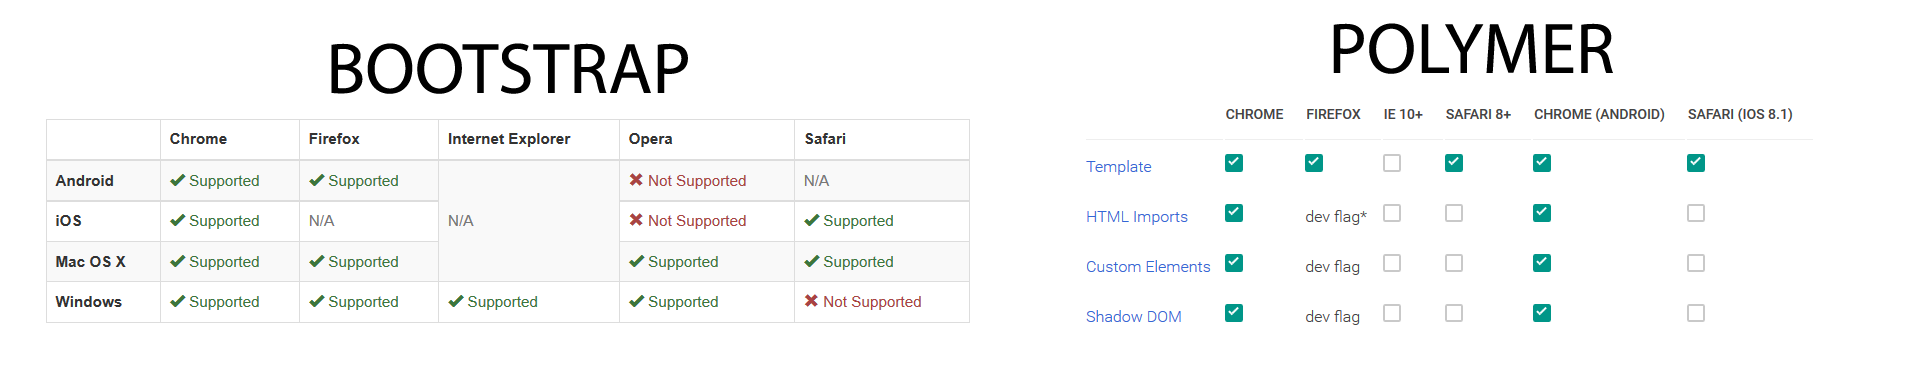
\includegraphics[width=0.48\textwidth]{p14}
  \end{center}
  \vspace{-20pt}
  \caption{Compatibilit\'e des technologies}
  \vspace{-10pt}
\end{wrapfigure}

Il s'agit sans doute de la premi\`ere chose \`a comparer. Bootstrap est support\'e par presque tout les navigateurs, Bootstrap n'est pas compatible avec Op\'era sur t\'el\'ephone et Safari sur Windows. Tandis que Polymer n'est compatible totalement qu'avec Google Chrome. Pour les autres navigateurs, Polymer est partiellement support\'e ou encore n'est pas du tout support\'e comme sur Internet explorer.En s'int\'eressant seulement \`a nos utilisateurs, on peux d\`es le d\'epart \'eliminer une des technologie. Polymer n'est clairement pas destin\'e \`a viser un large public. Notons de plus que les d\'eveloppeur de Mozilla Firefox ont d'ores et d\'ej\`a annonc\'e qu'il ne ferait aucun effort pour que leur navigateur supporte Polymer.\\

\subsection{Documentation}

La documentation est aussi un point fondamentale d'une technologie. Elle permet de faire la liason entre les utilisateurs et les nouvelles m\'ethodes de programmation. Sur Bootstrap, la documentation est claire et concise avec \`a chaque fois un exemple claire et simple \`a comprendre. Sur Polymer, ce point est mauvais. J'ai pass\'e de long moment \`a arpenter la documentation pour trouver certaines informations essentielles, ce qui repr\'esente une perte de temps non n\'egligeable. Par exemple, le point d'ancrage du nouveau composant est indiqu\'e par l'utilisation de la balise <content> dans le nouveau module. Cette information fondamentale ne se retrouve pas sur les exemples de base sur l'API (Application Program Interface) de Polymer.

\subsection{Vitesse de chargement}

\begin{wrapfigure}{l}{0.5\textwidth}
  \vspace{-25pt}
  \begin{center}
    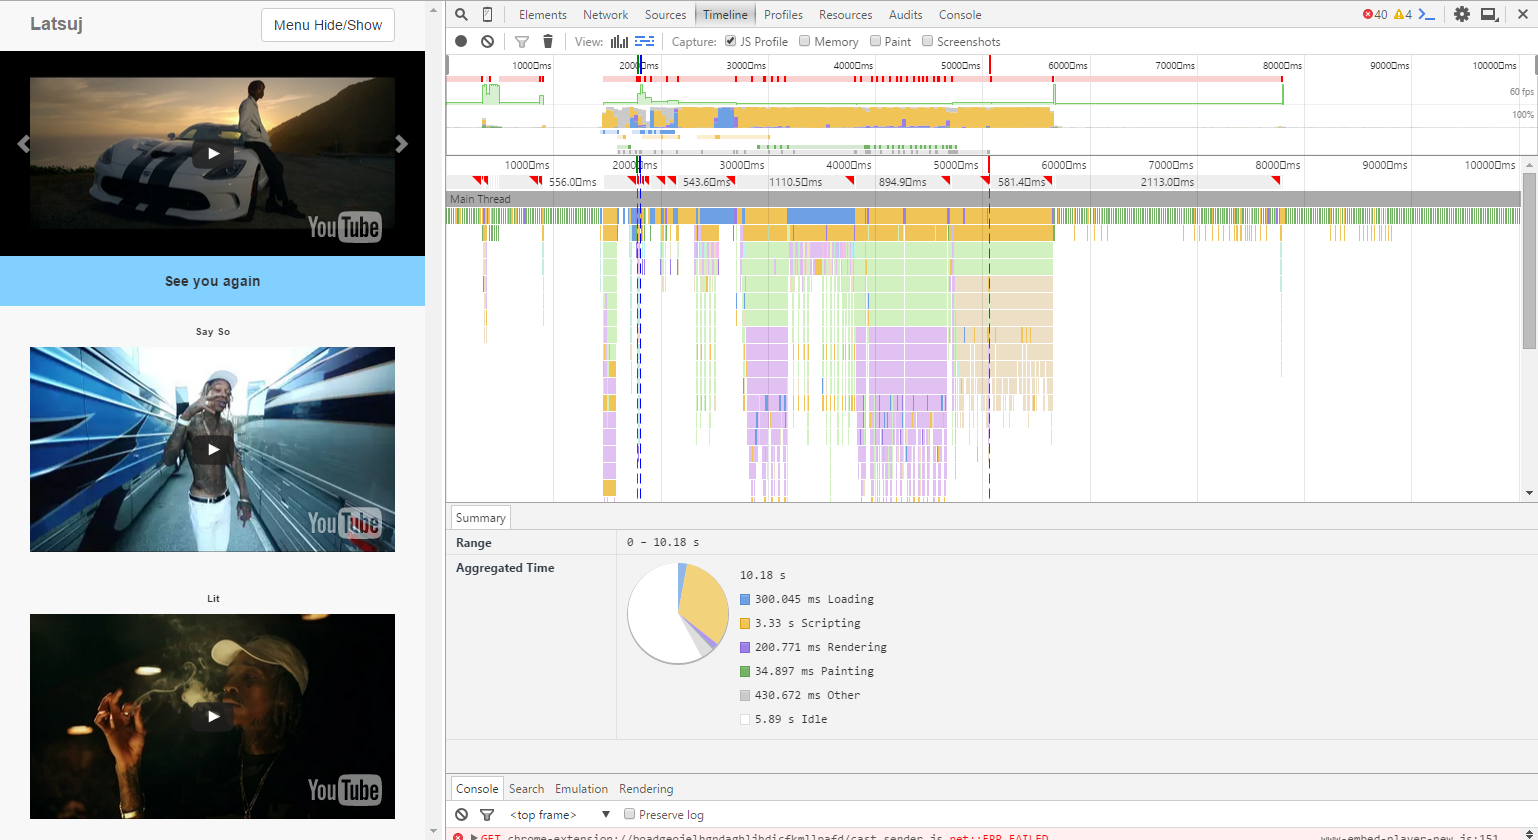
\includegraphics[width=0.48\textwidth]{p15}
  \end{center}
  \vspace{-20pt}
  \caption{Compatibilit\'e des technologies}
  \vspace{-10pt}
\end{wrapfigure}

En terme de performance, j'ai utilis\'e la fen\^etre de degoguage de Google Chrome pour savoir la vitesse d'\'ex\'ecution de nos deux technologies. Les deux site donnant le m\^eme r\'esultat, il serait normal de croire que le temps n\'ecessaire pour que le site soit pr\^et pour l'utilisateur soit identique. Malheuresement, ce n'est pas le cas. Pour Bootstrap, leur script est charg\'e en 3,33 secondes en moyenne tandis que celui de Polymer met 6,2 en moyenne. Ensuite, celui de Polymer doit effectuer ses traitements pour tranformer les \'el\'ements. Tout ceci a \'evidemment un cout en terme de performance. Avec Polymer, le site met en moyenne 400 ms pour apparaitre tandis qu'avec Bootstrap, cela tombe \`a 200 ms. L\`a encore, Polymer est encore en dessous de Bootstrap.

\newpage
\section{Comment teste-t-on les capacit\'es d'adaptations ?}

\subsection{Outils de test}

\hspace*{0.6cm}Pour tester l'affichage et l'adapatation de nos \'el\'ements \`a la fen\^etre, il existe plusieurs voies envisageables. J'ai utilis\'e plusieurs d'entre elle pour effectuer mes tests. La premi\`ere m\'ethode a \'et\'e de modifier la taille de la fen\^etre sous windows.\\

\begin{wrapfigure}{l}{0.5\textwidth}
  \vspace{-25pt}
  \begin{center}
    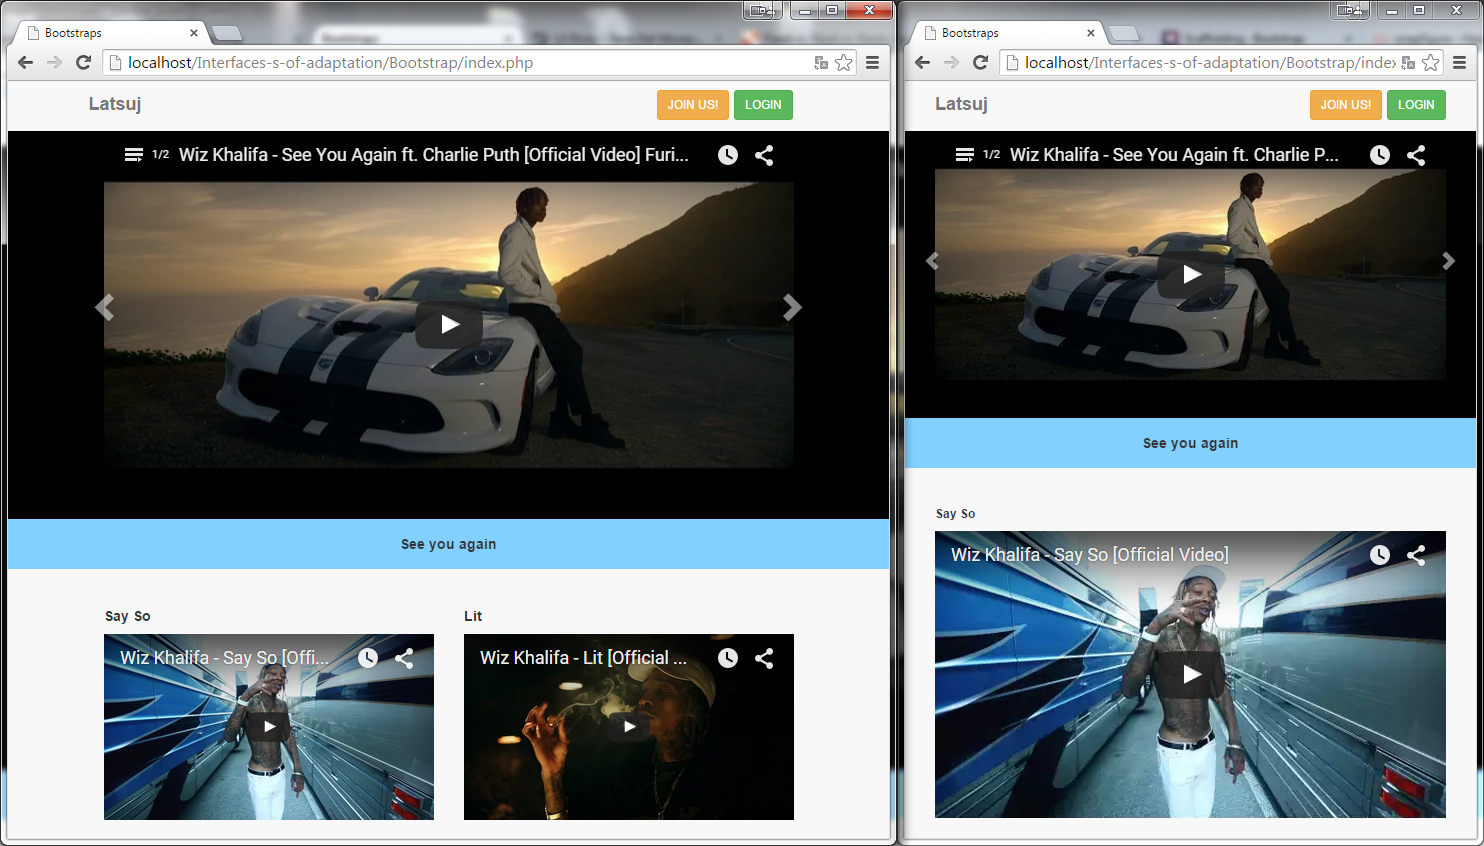
\includegraphics[width=0.48\textwidth]{double}
  \end{center}
  \vspace{-20pt}
  \caption{Redimensionnement de la fen\^etre sous windows}
  \vspace{-10pt}
\end{wrapfigure}

L'exemple de la figure 14 montre le site \`a deux dimensions diff\'erentes. Comme on peux le voir, le site s'adapte bien \`a la largeur de la fen\^etre. Sur la gauche, le site est plus grand. La taille plus grande permet de mettre deux clips vid\'eos l'un \`a cot\'e de l'autre. Sur la droite, le site est plus petit et ne permet de n'afficher qu'un clip vid\'eo par ligne. Les autres \'el\'ements quant \`a eux se redimensionne pour s'adapter \`a la page. J'ai r\'ealis\'e cette op\'eration avec chacun des navigateurs avec Bootstrap. Le r\'esultat obtenue est le m\^eme sur chacun des navigateurs. Avec Polymer, on ne peux test\'e qu'avec quelques navigateurs d\`u au probl\`eme de compatibilit\'e que j'ai \'evoqu\'e pr\'ec\'edemment.\\

\begin{wrapfigure}{r}{0.5\textwidth}
  \vspace{-25pt}
  \begin{center}
    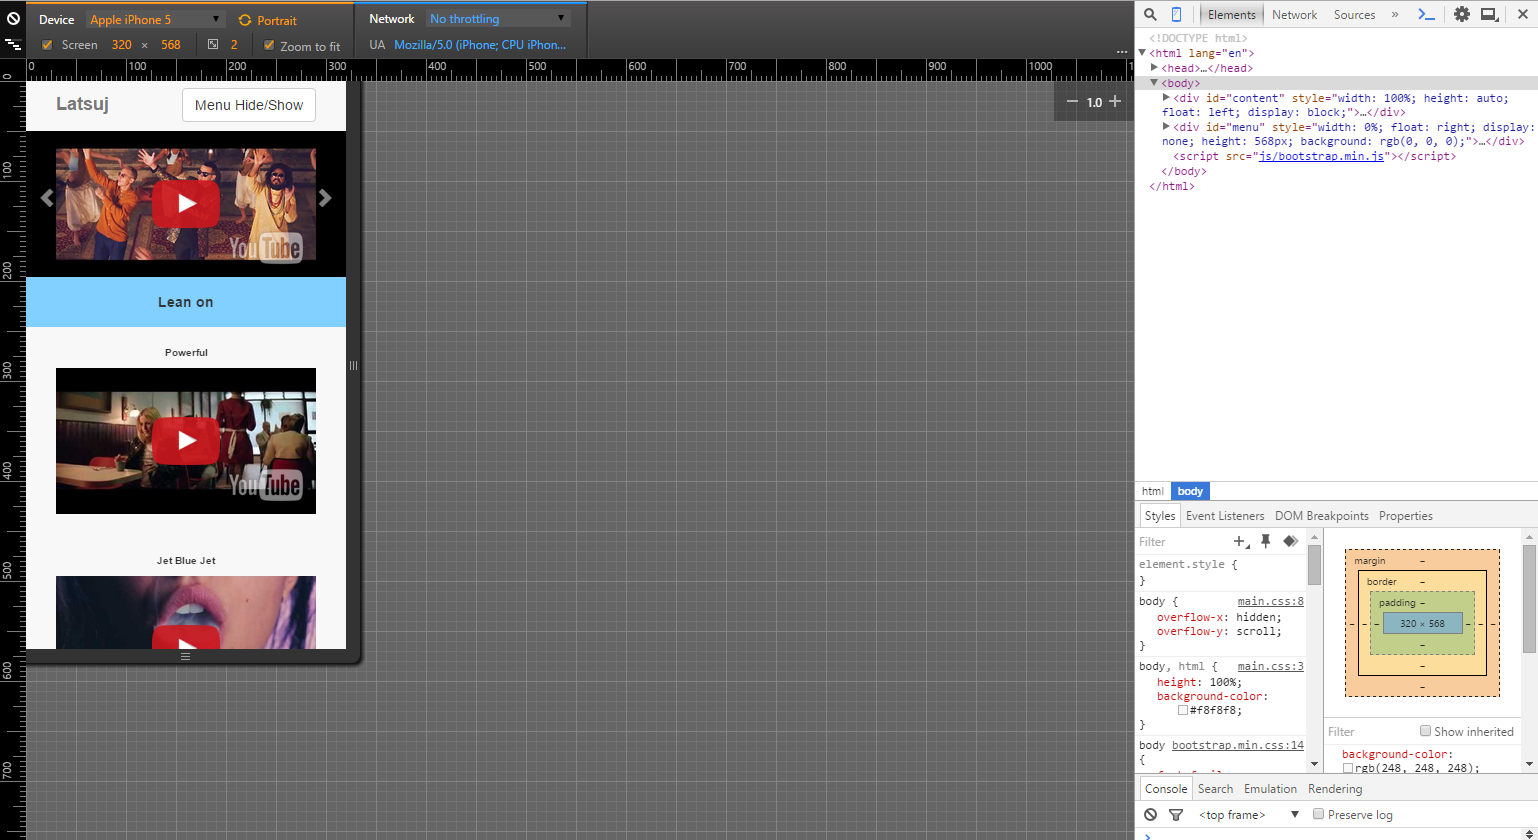
\includegraphics[width=0.48\textwidth]{p16}
  \end{center}
  \vspace{-20pt}
  \caption{Test au format iphone 5}
  \vspace{-10pt}
\end{wrapfigure}

Pour test\'e l'adaptation sur des appareils en particuliers, Google Chrome dispose d'un outil redimensionnant la fen\^etre \`a la dimension exacte d'un appareil en particulier. J'ai utilis\'e cet outil pour voir le r\'esultat sous diff\'erentes tablettes et t\'el\'ephones actuellement sur le march\'e. Pour activer cet option sous le navigateur, il suffit d'appuyer sur F12 puis le bouton repr\'esentant un t\'el\'ephone nomm\'e \og toggle device mode \fg{}.
\vspace{0.5cm}\\
\begin{wrapfigure}{l}{0.5\textwidth}
  \vspace{-25pt}
  \begin{center}
    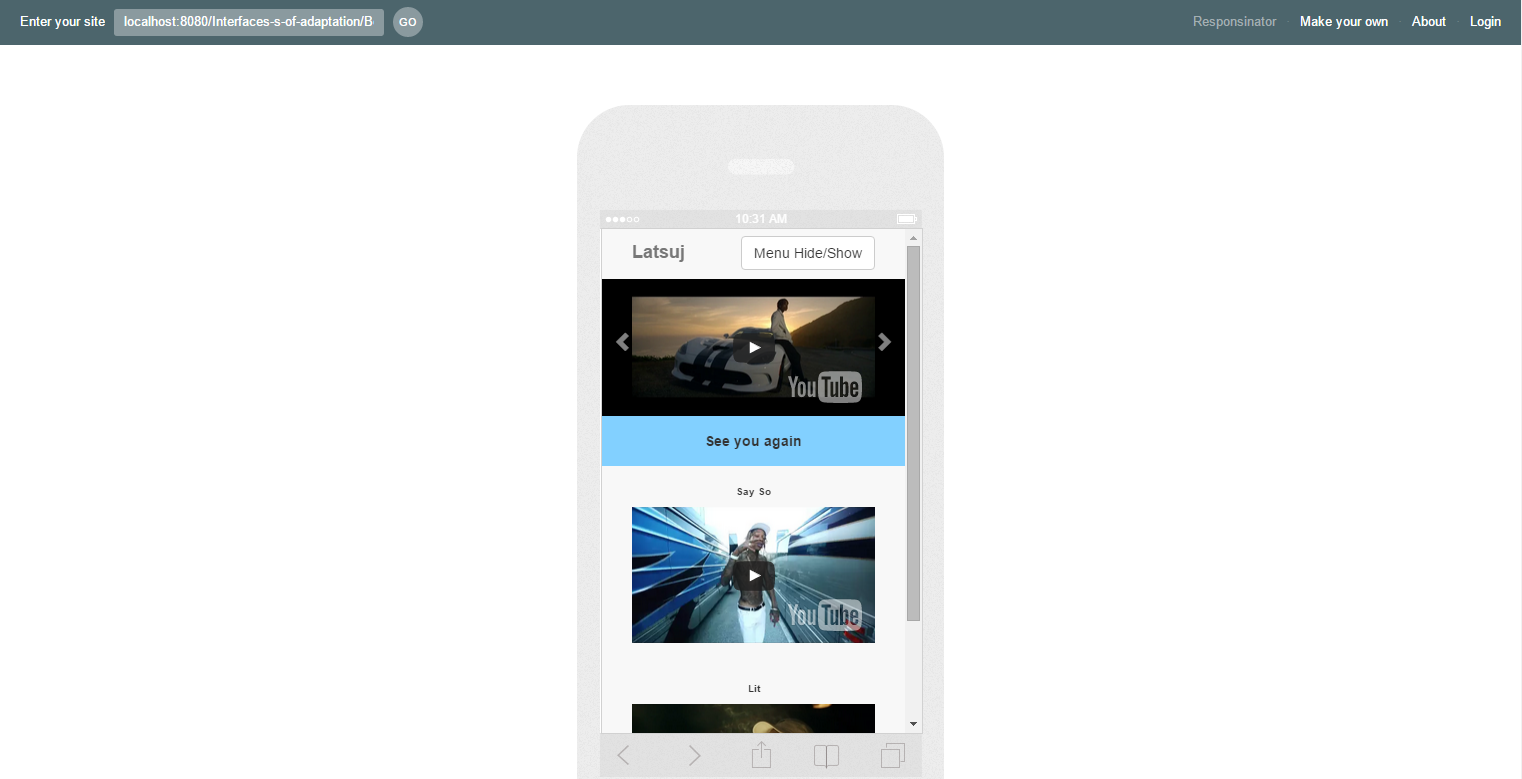
\includegraphics[width=0.48\textwidth]{p17}
  \end{center}
  \vspace{-20pt}
  \caption{Responsinator.com}
  \vspace{-10pt}
\end{wrapfigure} 

Il est aussi possible de passer par des sites qui permettent de tester l'adaptation de nos sites comme responsinator.com. J'ai aussi test\'e mon site sous cet \'el\'ement. On voit sur ce site un grand ensemble d'appareil avec notre site \`a l'int\'erieur. Le seul probl\`eme de cette m\'ethode est qu'il faut charger X fois le m\^eme site, ce qui peut s'av\'erer plutot long si le site en question est relativement lourd.\\

\subsection{\'El\'ements adaptatifs}

L'ensemble du site contient des \'el\'ements qui s'adaptent \`a la largeur de la fen\^etre. Que ce soit le menu, la vid\'eo principale, les images, le texte, chaque \'el\'ement \`a sa propre fa\c{c}on de se positionner, de se redimensionner suivant la largeur de la fen\^etre.

\newpage
\section{Documentations, Outils, liens utiles} 

\textbf{Wikip\'edia}\\
Le site d'o\'u j'ai d\'emarr\'e mes recherches, il contient une bonne d\'efinition des sites RWD.\\
\textit{https://fr.wikipedia.org/wiki/Site\_web\_adaptatif}
\vspace{0.5cm}\\
\textbf{What is a responsible web design ?}\\
Les liens suivant sont les articles ou vid\'eos que j'ai analys\'e pour \'ecrire ce rapport.\\
\textit{https://www.youtube.com/watch?t=133\&v=iSY38POjLYc}
\vspace{0.5cm}\\
\textbf{Ethan Marcotte}\\
Le site du createur du RWD qui montre la diff\'erence entre un site adpatable et un site responsive.\\
\textit{http://alistapart.com/d/responsive-web-design/ex/ex-site-flexible.html}\\
\textit{http://alistapart.com/d/responsive-web-design/ex/ex-site-linearize.html}
\vspace{0.5cm}\\
\textbf{Responsible typesetting}\\
Un article qui traite du responsible typesetting.\\
\textit{http://blog.line0.eu/responsible-typesetting/}
\vspace{0.5cm}\\
\textbf{Fitt's law}\\
La description de la loi de Fitt\\
\textit{https://en.wikipedia.org/wiki/Fitts's\_law}\\
\textit{http://webdesign.tutsplus.com/articles/applying-fitts-law-to-mobile-interface-design--webdesign-6919}
\vspace{0.5cm}\\
\textbf{Media queries}\\
Les medias queries sont int\'erressants mais limit\'es. Le futur serait plutot du cot\'e des \'el\'ements queries.\\
\textit{http://ianstormtaylor.com/media-queries-are-a-hack/}\\
\textit{http://www.smashingmagazine.com/2013/06/media-queries-are-not-the-answer-element-query-polyfill/}\\

\newpage
Mais cela n'est qu'un hack qui permet de faire ce que je d\'esire. On peux le faire mais on ne devrais pas le faire. Le gros probl\`eme ici est que ce code est non maintenable. Si jamais je changeais de point de rupture par exemple, je devrais changer la valeur de ce m\'edia query. Si il n'y a que celui-l\`a, ce n'est trop long et fatiguant. Mais si le projet a quelques milliers de modules, cela risque d'\^etre tr\`es long.



\newpage


Ne pas oublier de detailler le changement de point de rupture.

Colorions chaque divisions de cette partie du site d'une couleur unique.
\begin{center}
\vspace{0.5cm}
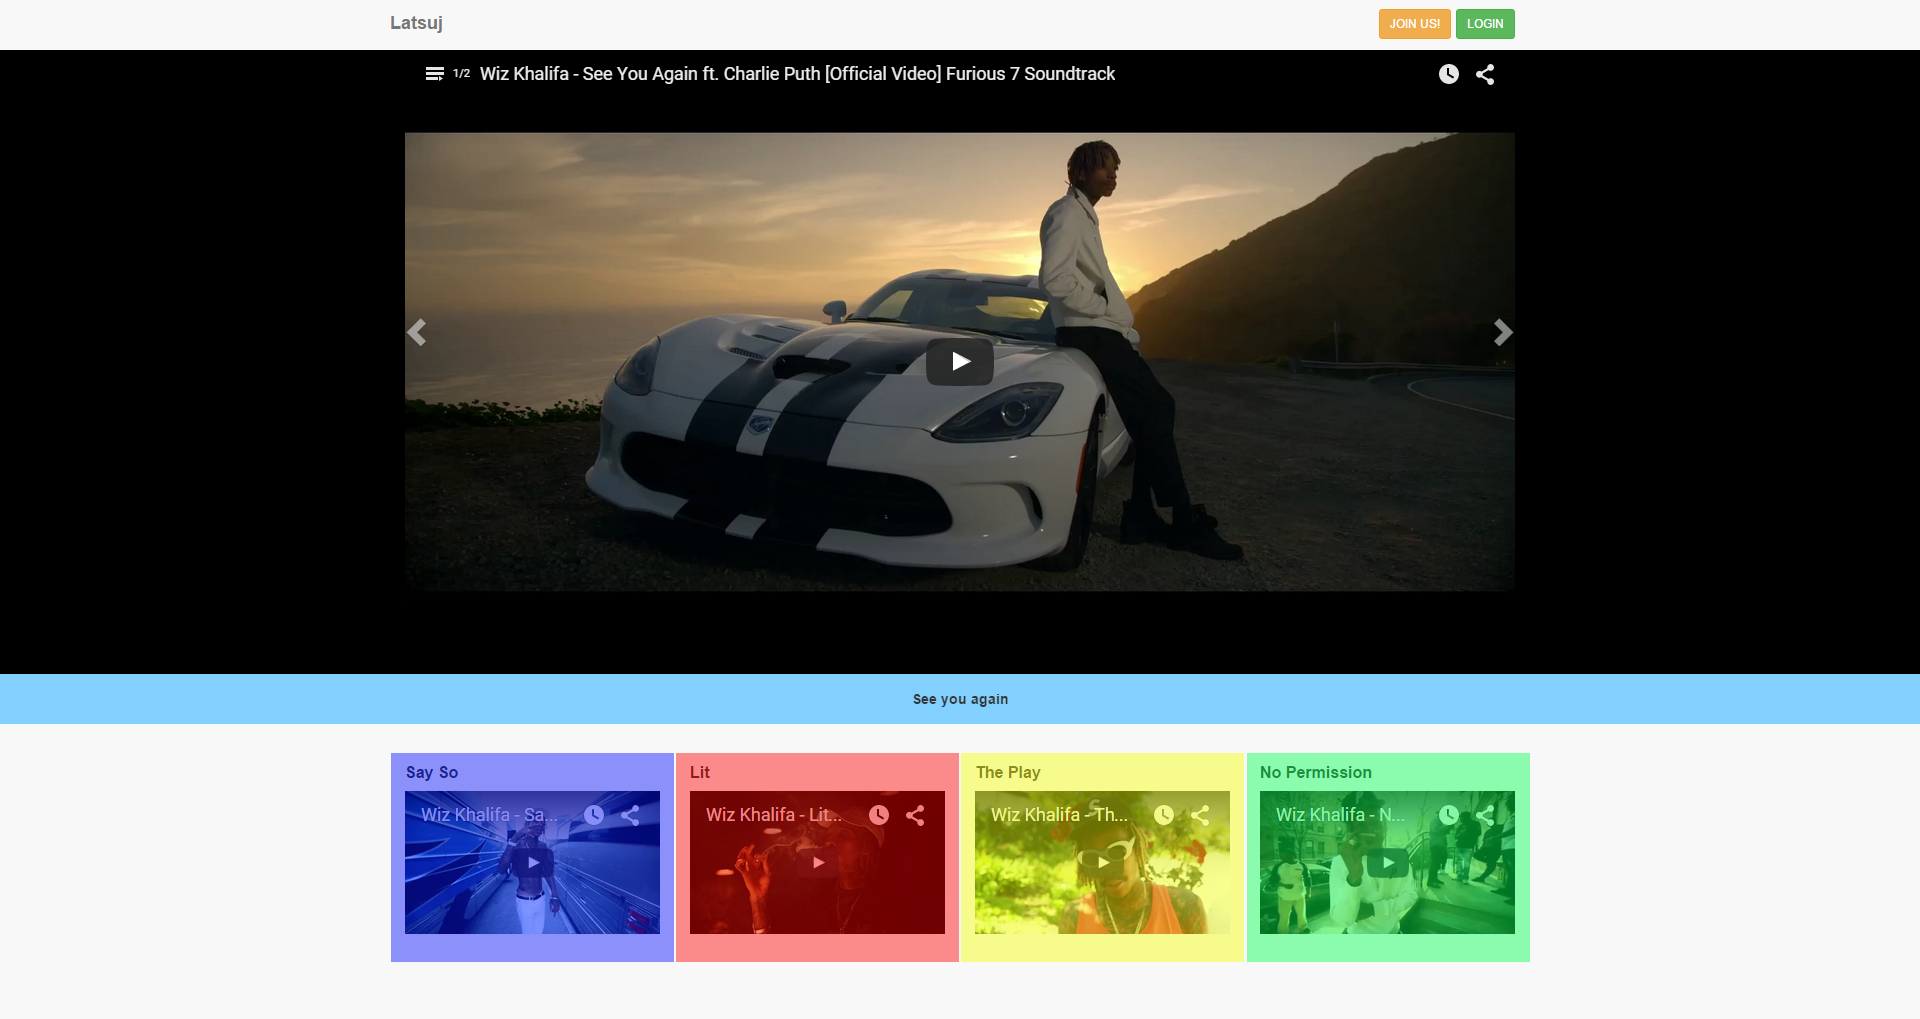
\includegraphics[width=0.8\textwidth]{pc4}
\vspace{0.5cm}
\end{center}
Si nous r\'eduisons la largeur de la fenetre, le contenu s'adaptera. Dans un premier temps, il n'y aura plus que deux blocs par ligne. Puis, si nous continuons de r\'eduire la fen\`etre, il n'y aura plus qu'un seul bloc par ligne et les deux derniers auront \'et\'e cach\'e.
\begin{center}
\vspace{0.5cm}
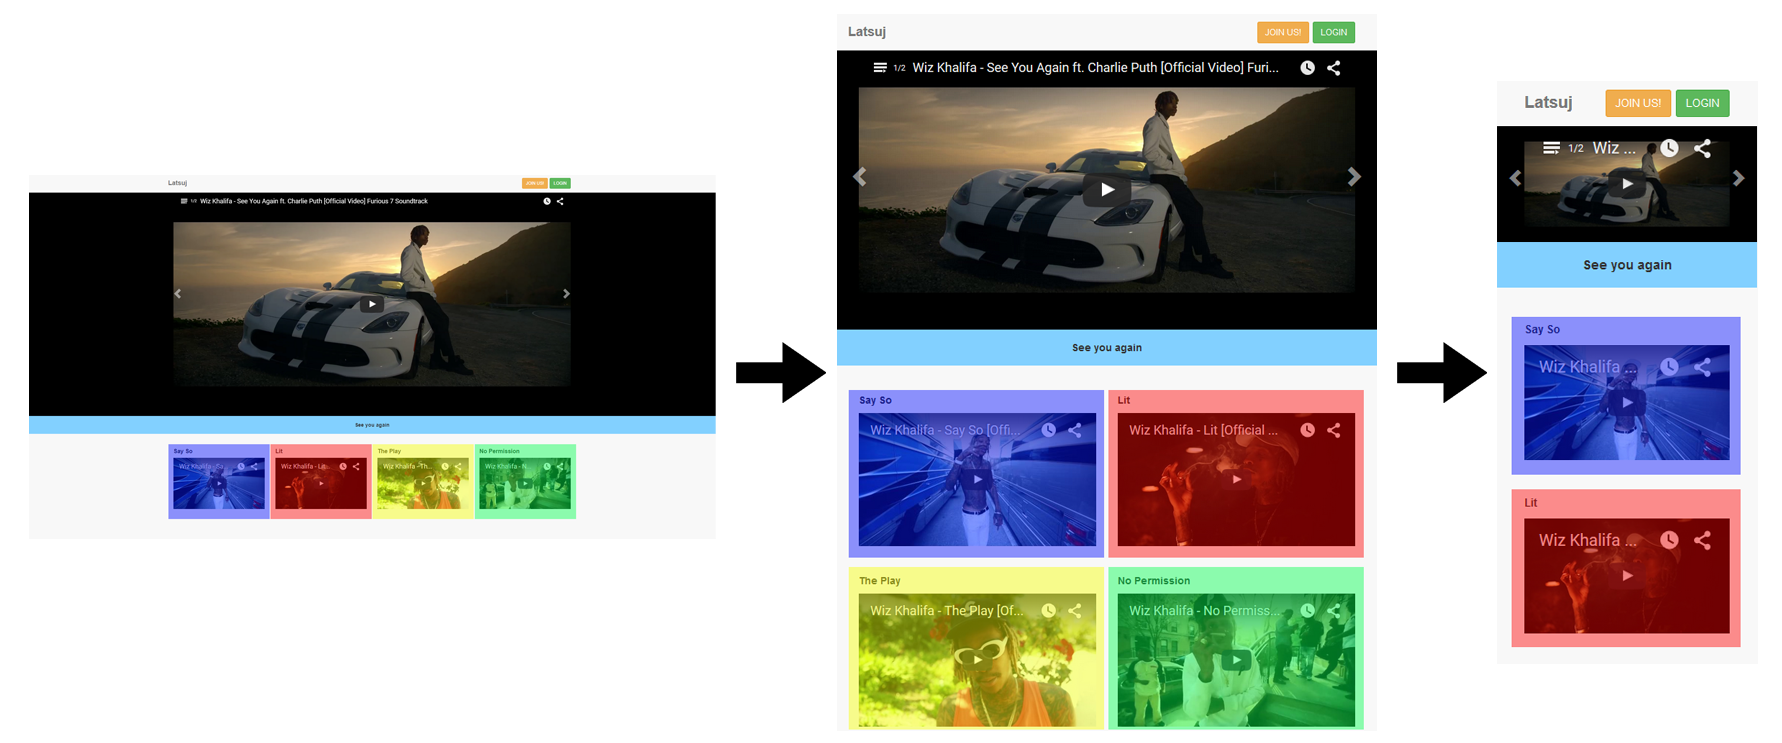
\includegraphics[width=0.8\textwidth]{pc7}
\vspace{0.5cm}\\
\end{center}

Le site s'adapte donc aux dimensions de notre appareil ou fen\`etre.\`A quoi cela peut-il bien servir ? Il serait plus adapté de se demander quels sont probl\`emes que cela r\'esout-il ? Comme on le voit autour de nous, les ordinateurs ne sont plus les seuls \'el\'ements ou gadgets nous entourant, ils existent maintenant une innombrable quantit\'e d'apareil informatique de tous types et de toutes dimensions. Il est important qu'un site internet ne laisse aucun utilisateur sur le bas cot\'e. Comme il est impensable de concevoir une application ou un site internet pour chaque appareil, il faut donc faire un site qui puisse s'adapter suivant les dimensions de l'appareil. 
\vspace{0.5cm}\\
Mais ce n'est pas tout, l'adaptation seul ne permet pas d'\'etablir ce que l'on peut appeler un site web adaptatif. Le cr\'eateur de cette vision, Mr. Ethan Marcotte, a implement\'e un site (\textit{http://alistapart.com/d/responsive-web-design/ex/ex-site-flexible.html}) qui s'adapte \`a la largeur de l'\'ecran. Cependant, il pointe du doigt certains d\'etails. Par exemple, lorsque l'on redimensionne la page, les \'el\'ements vont bel et bien se redimensionner mais les images et le texte \`a tr\`es basse r\'esolution deviendront illisible. Il faut donc que les \'el\'ements se repositionnent dans la page afin que le contenue soit lisible et agr\'eable \`a arpenter pour l'utilisateur. C'est pourquoi dans l'exemple ci-dessus, le nombre de bloc par ligne d\'ecroit au fur et \`a mesure que l'on r\'eduit la fen\^etre.
\vspace{0.5cm}\\

Le site est aussi \textit{responsible typesetting}. La taille en pixel du texte varie suivant la taille de la fen\^etre. Pour l'utilisateur, il est sans aucun doute plus agr\'eable de pouvoir lire les paroles d'une chanson phrase par phrase. Or, si la taille du texte restait la m\^eme pour toutes dimensions de fen\`etre, soit le texte serait illisible \`a une grande r\'esolution, soit le site serait incommode \`a basse r\'esolution. Pour r\'esoudre ce probl\`eme, une proportions a \'et\'e sp\'ecifier pour l'ensemble des textes suivant la largeur de la fen\`etre ou de l'appareil. Sur le site, on retrouve cette particularit\'e sur plusieurs titres et sur les paroles comme nous pouvons le constater ci-dessous. \`A gauche, on retrouve les paroles des chansons sur t\'el\'ephone portable tandis que \`a droite, on retrouve les m\^emes paroles \'ecrite avec une plus grande police sur tablette.
\begin{center}
\vspace{0.5cm}
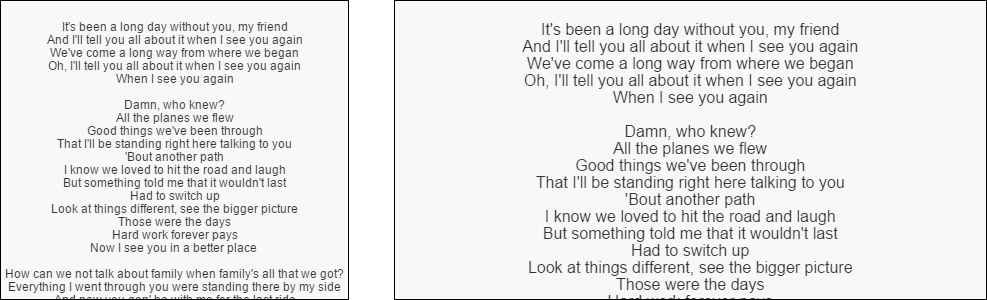
\includegraphics[width=0.8\textwidth]{textes}
\vspace{0.5cm}\\
\end{center}

\newpage

\hspace*{0.6cm}Pourquoi ais-je supprim\'e les deux derniers blocs sur la navigation \`a basse r\'esolution ? Ce n'est pas une d\'ecision anodine. En supprimant ces deux blocs, j'am\'eliore l'exp\'erience de l'utilisateur sur deux aspects.\\
\begin{wrapfigure}{r}{3cm}
\vspace{-13pt}
\centering
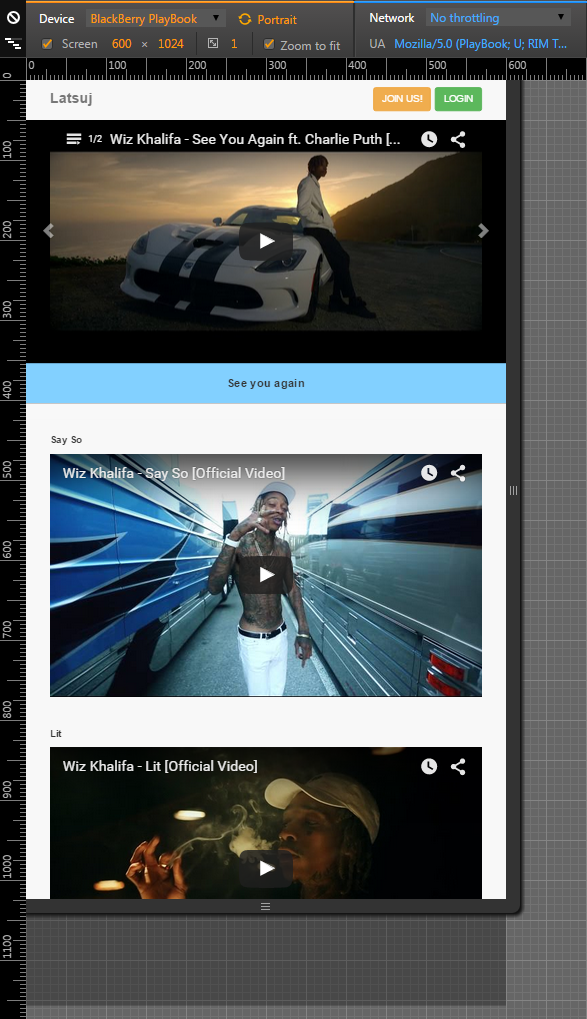
\includegraphics[width=3cm]{blackberry}
\caption{\textit{Affichage du site sous BlackBerry (via Google Chrome).}}
\end{wrapfigure} 
{\hspace*{0.6cm}L'un est purement li\'e \`a la technologie, il est rare d'avoir un t\'el\'ephone branch\'e en Ethernet. Ceci implique que le d\'ebit moyen d'un utilisateur sur t\'el\'ephone est souvent inf\'erieur \`a celui d'un utilisateur sur ordinateur. J'\'evite ainsi \`a l'utilisateur sur t\'el\'ephone de charger trop d'informations qui n'appartiennent pas au contenue principal de la page. Ce ne sont que des publicit\'es pour les autres musiques du m\^eme chanteur. Deuxi\`emement, et c'est sans doute le point le plus important, suivant \textbf{la loi de Fitt}, que je sois sur t\'el\'ephone ou ordinateur l'indice de difficult\'e doit rest\'e le m\^eme. La loi calcul donne un indice de difficult\'e par rapport au temps requis pour aller rapidement d'une position de d\'epart \`a une zone finale de destination. L'utilisateur doit arriver avec la m\^eme rapidit\'e et la m\^eme facilit\'e aux diff\'erentes parties du site. Si l'on regarde l'image sur la droite qui repr\'esente le site sur un t\'el\'ephone BlackBerry, on remarque que le temps pour parvenir \`a la derni\`ere vid\'eo en rapport avec le chanteur est aussi rapide sur le t\'el\'ephone que sur ordinateur. Certes ce n'est pas la m\^eme, mais cela reste la derni\`ere vid\'eo. Si j'avais juste r\'earrang\'e les choses, il aurait d'abord fallu descendre pour arriver \`a la derni\`ere vid\'eo. Cela ne para\^it pas beaucoup plus compliqu\'e mais sans cela, le site se retrouverait complexifi\'e d'apr\`es la loi de Fitts.}\\

\newpage
\section{Difficult\'es rencontr\'es}
\hspace*{0.6cm}Le premier probl\`eme rencontr\'e fut lorsque que j'essaya de coder une balise div de telle mani\`ere que celle-ci remplisse enti\`erement l'espace de l'application. Cette chose extr\`emement simple n'est pourtant pas impl\'ement\'e dans Bootstrap 3.0 et les versions sup\'erieur alors que cela se trouvait dans les versions ant\'erieur avec la class span. Apr\'es de longue recherches, il apparait donc impossible en pur Bootstrap de remplir un div \`a cent pour cent de la balise parent.De ce fait, j'ai du modifi\'e le CSS pour r\'ealiser le remplissage de la page. Pourquoi un tel choix des d\'eveloppeur de bootstrap ?

margin-bottom : Seriously ?

Compatibilite : WTF polymer !

min-height ? WTF do not work !OK parce que tous ces putain d'elements sont en inline et non en block...Ok l'erreur

Suivre un ordre pour appeler les modules au depart, les enfant en premier.

encapsulation des elements ? content :X Merci la doc....pourrie.

Le carousel une horreur sur Polymer....

Bootstrap, position fixed et col does not work.

J'ai du recompiler le bootstrap.

\section{Simple trouvaille d'optimisation}
En farfouillant sur les documentations de Bootstrap, je suis tomb\'e sur une optimisation qui a retenu mon attention. Une chose simple et pourtant efficace que je ne faisait pas moi non plus. Les developpeurs de Bootstrap mettent toujours les scripts javascript en fin de page afin d'accelerer le chargement de la page. Cela peut paraitre stupide comme remarque mais je tiens \`a m'en souvenir, j'en fait donc par dans mon document.

Petite astuce, enlever les ; sur le dernier elements de css pour gagner un caractere de lecture.

\end{document}
